% !TeX root = ../thuthesis-example.tex

\chapter{中性粒细胞候选必需蛋白筛选与特征分析}

\section{基于 PES 评分的蛋白功能分群}

本研究旨在识别中性粒细胞执行特定功能时不可或缺的候选蛋白。通过构建 Human-level 与 Immune-level 双模型评分体系，旨在从群体进化约束与细胞情境依赖两个维度对蛋白必需性进行定量评估。

对两模型输出的 PES 进行整体相关性分析。如图~\ref{fig:model_comparison}(a) 所示，横轴与纵轴分别是 $PES_{\text{human}}$ 和 $PES_{\text{immune}}$。统计分析表明，两模型输出 PES 的 Pearson 相关系数仅为 $r = 0.073$ ($p < 0.001$)。散点图呈现高度弥散的分布特征，而非向 $y=x$ 对角线集中。这种极低的相关性说明，蛋白在物种水平受到的进化压力与其在特定免疫细胞中的生存贡献之间并不存在显著的线性对应关系。

通过 $PES=0.8$ 的阈值线进行划分，可以观察到明显的 两个模型的蛋白 PES 分布偏离现象：
\begin{itemize}
    \item 散点图中右下区域集中了大量在群体层面表现为高必需性但免疫细胞层面非必需的蛋白。由于中性粒细胞是高度分化且不具备增殖能力的终末细胞，许多维持细胞周期或基础发育的蛋白在其特定的生理周期内表现出较低的依赖权重，呈现出明显的背景特异性。
    \item 与之对应，左上区域存在大量群体层面在进化上相对耐受、但在 Immune-level 情境下得分显著升高的蛋白。这部分蛋白反映了细胞内部存在一套区别于基础生存需求的条件性功能调节网络，体现了必需性得分随功能情境变化的动态调整。
\end{itemize}
这说明，Human-level 与 Immune-level 模型在必需性判定上存在显著的维度差异。
位于左上象限的蛋白集合虽然在广义进化背景下表现出较高的功能冗余性，但在中性粒细胞特定的生理语境下却具有较高的依赖得分。这种预测结果的非一致性直观地展示了两模型在捕捉情境特异性必需基因时的差异化侧重。这证实了综合考虑双模型得分的必要性，并为后文中确立分群阈值及功能集合划分提供了依据。

在证实双模型预测结果存在显著差异后，需进一步量化其分布规律，以确立科学的候选蛋白筛选标准。图~\ref{fig:model_comparison}(c) 展示了两模型在全基因组范围内的得分密度分布情况。$PES_{\text{human}}$ 呈现出典型的双峰分布格局：在 $PES \approx 0.1$ 附近存在一个代表非必需蛋白的宽峰，而在 $PES > 0.8$ 的高分区间则形成了一个显著的尖峰。这种分布态势反映了 Human-level 模型能够清晰地界定出进化受限程度极高的核心必需基因，即那些维持生物体基本生存的基因集合。

相比之下，Immune-level 模型的分布特征呈现出明显的重心偏移，其高分区间的峰值显著平缓。这种分布形态的差异暗示，在 Immune-level 所表征的高应激功能情境下，蛋白的功能依赖性高度集中于少数核心通路。即大部分蛋白对该情境下的功能维持贡献较低，仅有极少数关键节点维持高水平权重。

为了准确界定高置信度必需蛋白的边界，进行了阈值敏感性分析。如图~\ref{fig:model_comparison}(b) 所示，随着 $PES$ 阈值从 0 逐渐提升至 1.0，两模型筛选出的蛋白数量表现出截然不同的衰减速率。值得注意的是，Immune-level 模型的筛选数量在 PES 从 0.2 提升至 0.6 的中等分值区间内经历了剧烈下降，这意味着大量具有中等进化保守性的蛋白并不会在该高应激功能情境下形成稳定依赖。随后在 $PES = 0.8$ 附近，曲线的下行斜率明显趋于平稳，进入了高得分的收敛平台区。

在相同的高阈值（$PES = 0.8$）水平下，Human-level 模型保留的蛋白规模远大于 Immune-level 模型，这表明 Immune-level 模型在高分区间施加了更严苛的筛选压力，能够更精准地富集那些在免疫情境下具有实质性功能贡献的分子。综合分布形态的峰值演变与敏感性曲线的拐点观测，本研究选定 $PES > 0.8$ 作为识别高置信度候选必需蛋白的阈值。该标准的建立，不仅在统计学上保证了候选集的严谨性，也为后续将蛋白精确划分为人类基础必需、免疫情境候选必需及共同必需三个功能集合提供了定量依据。

\begin{figure}[!htbp]
    \centering
    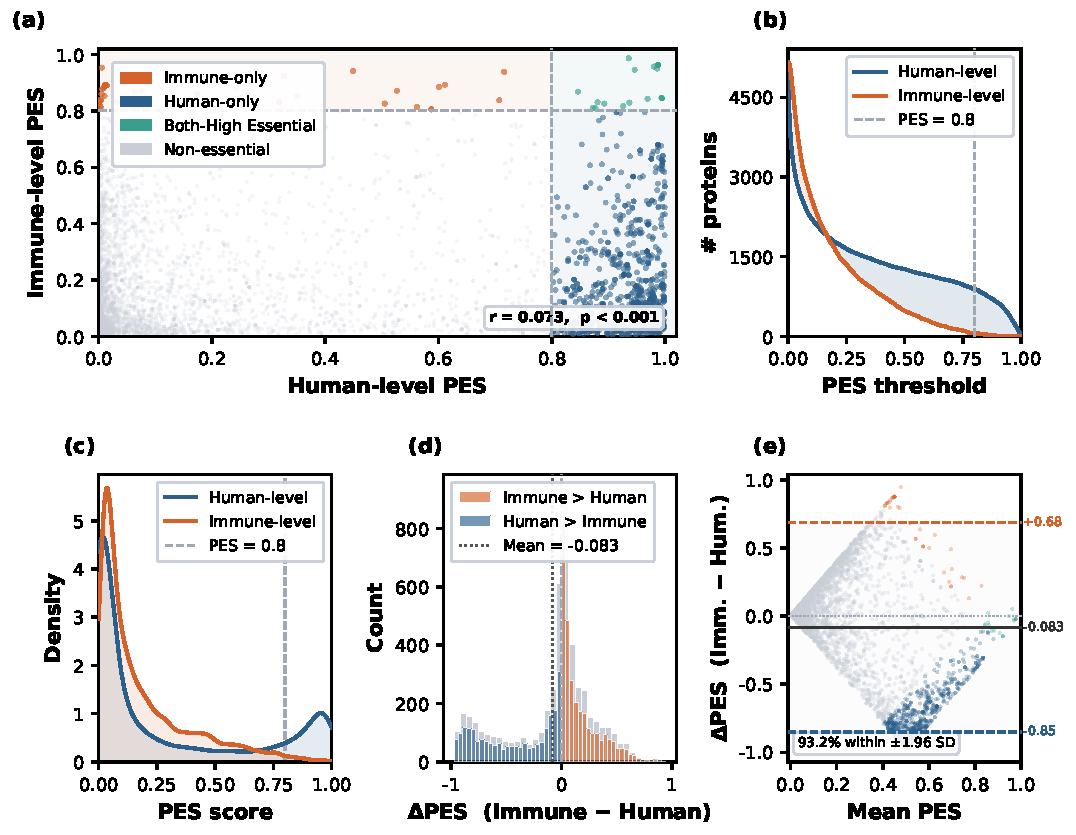
\includegraphics[width=1\linewidth]{figures/model_comparison.pdf}
    \caption[Human-level 模型与 Immune-level 模型的 PES 得分对比分析]{Human-level 模型与 Immune-level 模型的 PES 得分对比分析，显示两模型在低分区间具有较高一致性，而在高依赖蛋白区域呈现显著分化。(a) 两模型输出 PES 的散点相关性分布；(b) 不同 PES 阈值下筛选蛋白数量的变化趋势；(c) 两模型在全基因组范围内的 PES 密度分布；(d) 跨模型得分差值 $\Delta$PES 的频率分布；(e) 基于 Bland--Altman 方法的一致性评估。}
    \label{fig:model_comparison}
\end{figure}

在确立筛选阈值后，需要通过统计学手段评估双模型预测效能的一致性与差异性。图~\ref{fig:model_comparison}(d) 展示两模型得分差值（$\Delta PES$）的频率分布。尽管分布均值 $-0.083$ 略微偏向负值，暗示 $PES_{\text{human}}$ 在整体水平上具有略高的得分倾向，但分布曲线呈现出明显的双侧对称长尾结构。这种长尾特征在定量层面证实了前文提及的预测差异：即存在相当比例的蛋白，其必需性评价在不同背景下发生了剧烈波动。这些处于分布末端的离群分子，正是解析中性粒细胞情境依赖性调控机制的关键切入点。

进一步采用更加通用的 Bland–Altman 方法对两模型的一致性进行深度评估，如图~\ref{fig:model_comparison}(e) 所示。约 93.2\% 的观测点落在 $\pm 1.96 SD$ 的一致性区间内，这说明双模型在全基因组水平的预测趋势具备统计学意义的可比性。然而，从散点形态随平均值演变的走势来看，观测点呈现出显著的“漏斗状”扩散态势。

具体而言，在低分区间（$PES \approx 0$），散点紧密围绕均值线分布，说明两模型对非必需蛋白的判定具有极高的共识；而随着平均 PES 值的增大，尤其是进入 $0.6-1.0$ 的高依赖区间后，预测差异显著放变大，大量观测点开始逼近甚至突破一致性界限。这种在高分区的差异放大现象并非源于随机误差，而是深刻反映了双模型在处理核心功能蛋白时逻辑维度的本质分歧。在低分区的“一致性”保证了模型的基准可靠性，而高分区的“分歧”则恰恰为锁定中性粒细胞特有的功能节点提供了关键线索。这种分布特征验证了单一模型在处理复杂细胞情境时的局限性，从而支撑了本研究采用双模型联合筛选策略的必要性。

综合上述分析，本研究基于 PES 构建蛋白分群标准，以 $PES > 0.8$ 作为高置信度必需蛋白判定阈值，并在 Human 与 Immune 两个维度上对蛋白进行归类：

\begin{itemize}
    \item \textbf{人类基础必需蛋白：} 定义为 $PES_{\mathrm{human}} > 0.8$ 且 $PES_{\mathrm{immune}} \le 0.8$。该类蛋白在种群层面高度受限，主要反映基础生存需求，构成个体生存的\mbox{基本框架}。
    \item \textbf{免疫情境候选必需蛋白：} 定义为 $PES_{\mathrm{immune}} > 0.8$ 且 $PES_{\mathrm{human}} \le 0.8$。该类蛋白在群体层面相对耐受，但在 Immune-level 所表征的高应激功能情境下表现出更强依赖性，体现出免疫情境相关的功能需求，具有潜在\mbox{靶点价值}。
    \item \textbf{共同必需蛋白：} 定义为 $PES_{\mathrm{human}} > 0.8$ 且 $PES_{\mathrm{immune}} > 0.8$。该类蛋白在两个层级均表现为高依赖，构成生命活动骨架。
    \item \textbf{共同非必需：}定义为 $PES_{\mathrm{human}} \le 0.8$ 且 $PES_{\mathrm{immune}} \le 0.8$。该类蛋白在两个层级中均未表现出显著依赖，由于其在免疫反应中的依赖性较低，本研究未进一步探讨该类蛋白。未来研究可以考虑在特定免疫应答或疾病状态下评估这些蛋白的潜在功能。
\end{itemize}

通过上述分群策略，本节实现了从模型预测结果到功能集合划分的转化，为后续候选必需蛋白的结构特征分析与功能机制研究奠定基础。

\section{免疫情境候选必需蛋白的理化特征分析}

中性粒细胞作为高度应激化的先天免疫效应细胞，其功能执行环境具有显著的物理化学压力特征，包括吞噬体快速酸化（pH 4.5--5.0）、ROS 爆发、蛋白酶富集以及高动态膜重塑过程。尤其在急性炎症应答中，免疫情境在中性粒细胞中的具体表现可归纳为氧化爆发增强和颗粒/溶酶体功能负荷升高。因此，若免疫情境候选必需蛋白承担该情境下的关键功能，其序列层面的理化属性理应呈现与此类环境压力相适应的系统性偏移。为验证该推断，本研究对免疫情境候选必需蛋白与人类基础必需蛋白在氨基酸组成及整体理化参数层面进行了系统比较分析。

通过图~\ref{fig:aa_composition}对氨基酸组成比例的精细化比较发现，免疫情境候选必需蛋白在残基水平经历了显著不同的系统性偏移。在碱性氨基酸中赖氨酸（Lys，K）比例显著增加（$\Delta +3.6\%$），而同为正电荷残基的精氨酸（Arg，R）增幅相对较小（$\Delta +1.6\%$）。由于 Lys 侧链具有更强的构象柔性，且常作为乙酰化、泛素化等关键翻译后修饰的受体，这种非对称性的电荷增加暗示免疫情境候选必需蛋白在跨膜信号传导与蛋白质降解调控中具有更高的灵活性。与此同时，疏水性残基如缬氨酸（Val，V）的比例有所上升（$\Delta +0.9\%$），而酸性残基（D, E）及极性不带电残基（N, Q）比例则呈现系统性下降。这种“增疏水、去极性”的趋势有利于在胞内高氧化压力的 ROS 环境下，构建更为致密的内部疏水核心，从而在化学层面减少蛋白主链受氧化损伤的风险。此外，具有高氧化敏感性的半胱氨酸（Cys，C）比例在免疫情境候选必需蛋白中有所降低，这一特征直接降低了蛋白发生非特异性氧化交联的可能性，增强了其在炎症微环境中的结构稳态。

\begin{figure}[!htbp]
    \centering
    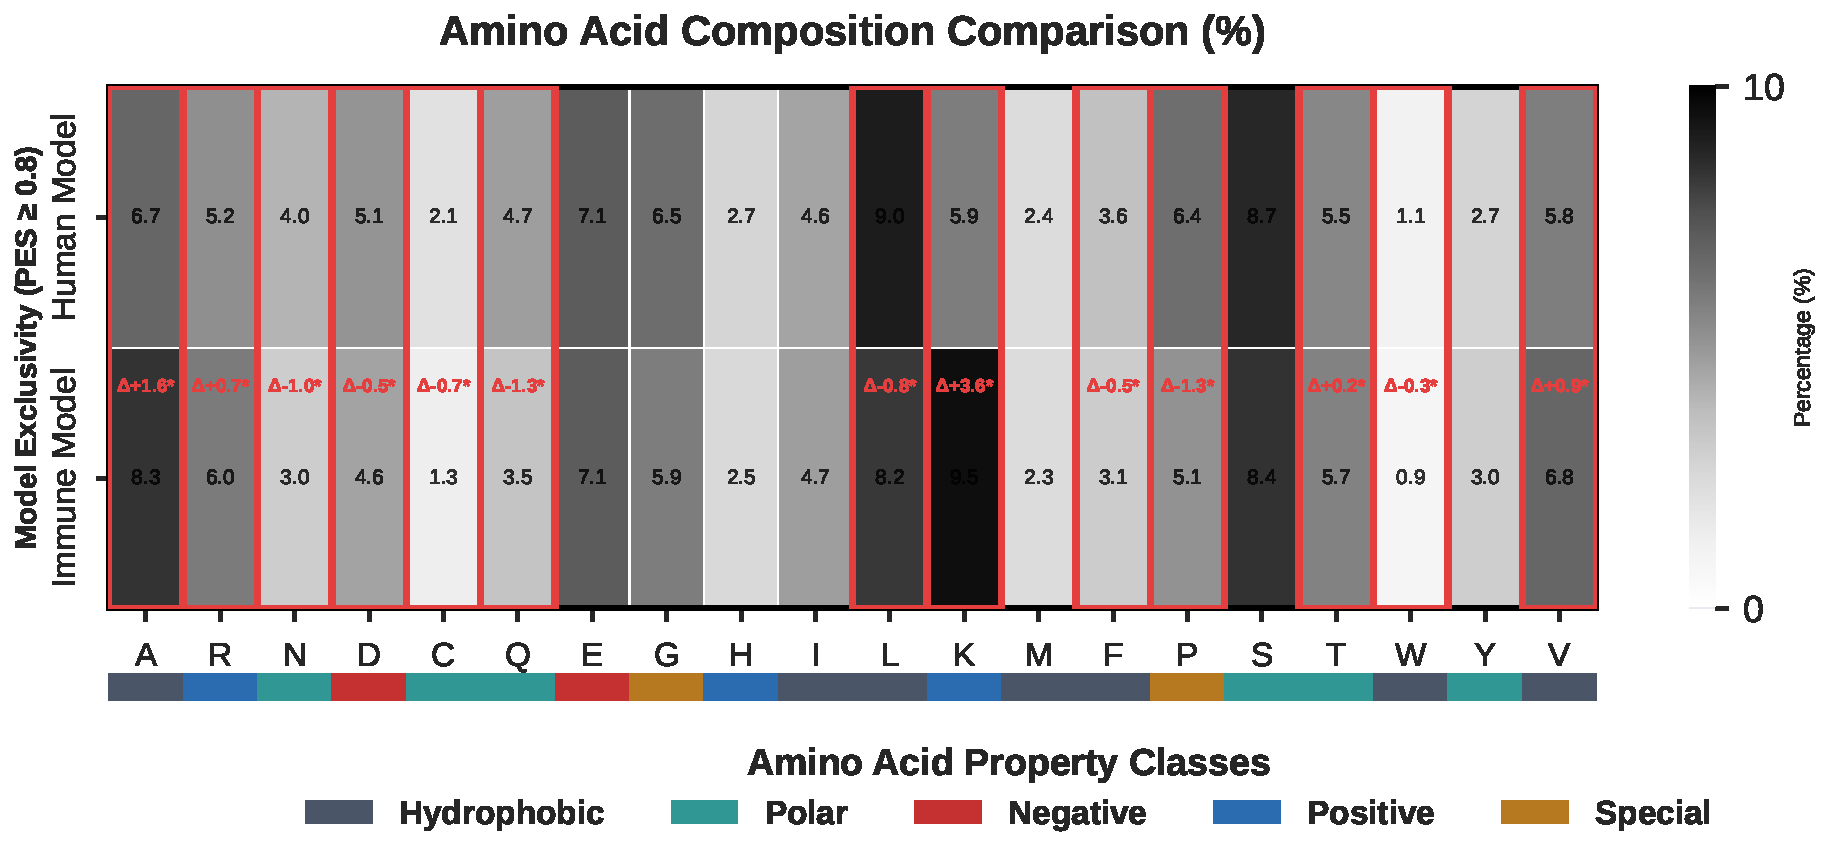
\includegraphics[width=0.98\linewidth]{figures/aa_composition.pdf}
    \caption[免疫情境候选必需蛋白与人类基础必需蛋白的氨基酸组成差异比较]{免疫情境候选必需蛋白与人类基础必需蛋白的氨基酸组成差异比较。该图按残基类别展示两类蛋白在氨基酸组成上的系统偏移，突出免疫情境候选必需蛋白在碱性残基增加、极性残基减少及疏水性增强等方面的整体趋势。}
    \label{fig:aa_composition}
\end{figure}

分析理化属性的统计分布特征进一步印证了上述序列水平的偏移。如图~\ref{fig:biophysical_features}(a) 所示，免疫情境候选必需蛋白的分子量显著低于人类基础必需蛋白（***$p<0.001$）。从分布曲线可以观测到，人类基础必需蛋白的分子量跨度极大，部分蛋白高达 500 kDa 附近，而免疫情境候选必需蛋白的分布则表现出明显的向小分子量偏移，高度集中在 100 kDa 以下的低分子量区间。这种“结构轻量化”趋势在生物学上具有双重意义：一方面，较短的肽链有助于在应急粒生成状态下缩短单分子的翻译耗时，实现免疫效应因子的快速动员；另一方面，小分子量蛋白通常拥有更简单的折叠路径，在极端应激环境下相比大型多畴蛋白更不易发生错误折叠。

\begin{figure}[!htbp]
    \centering
    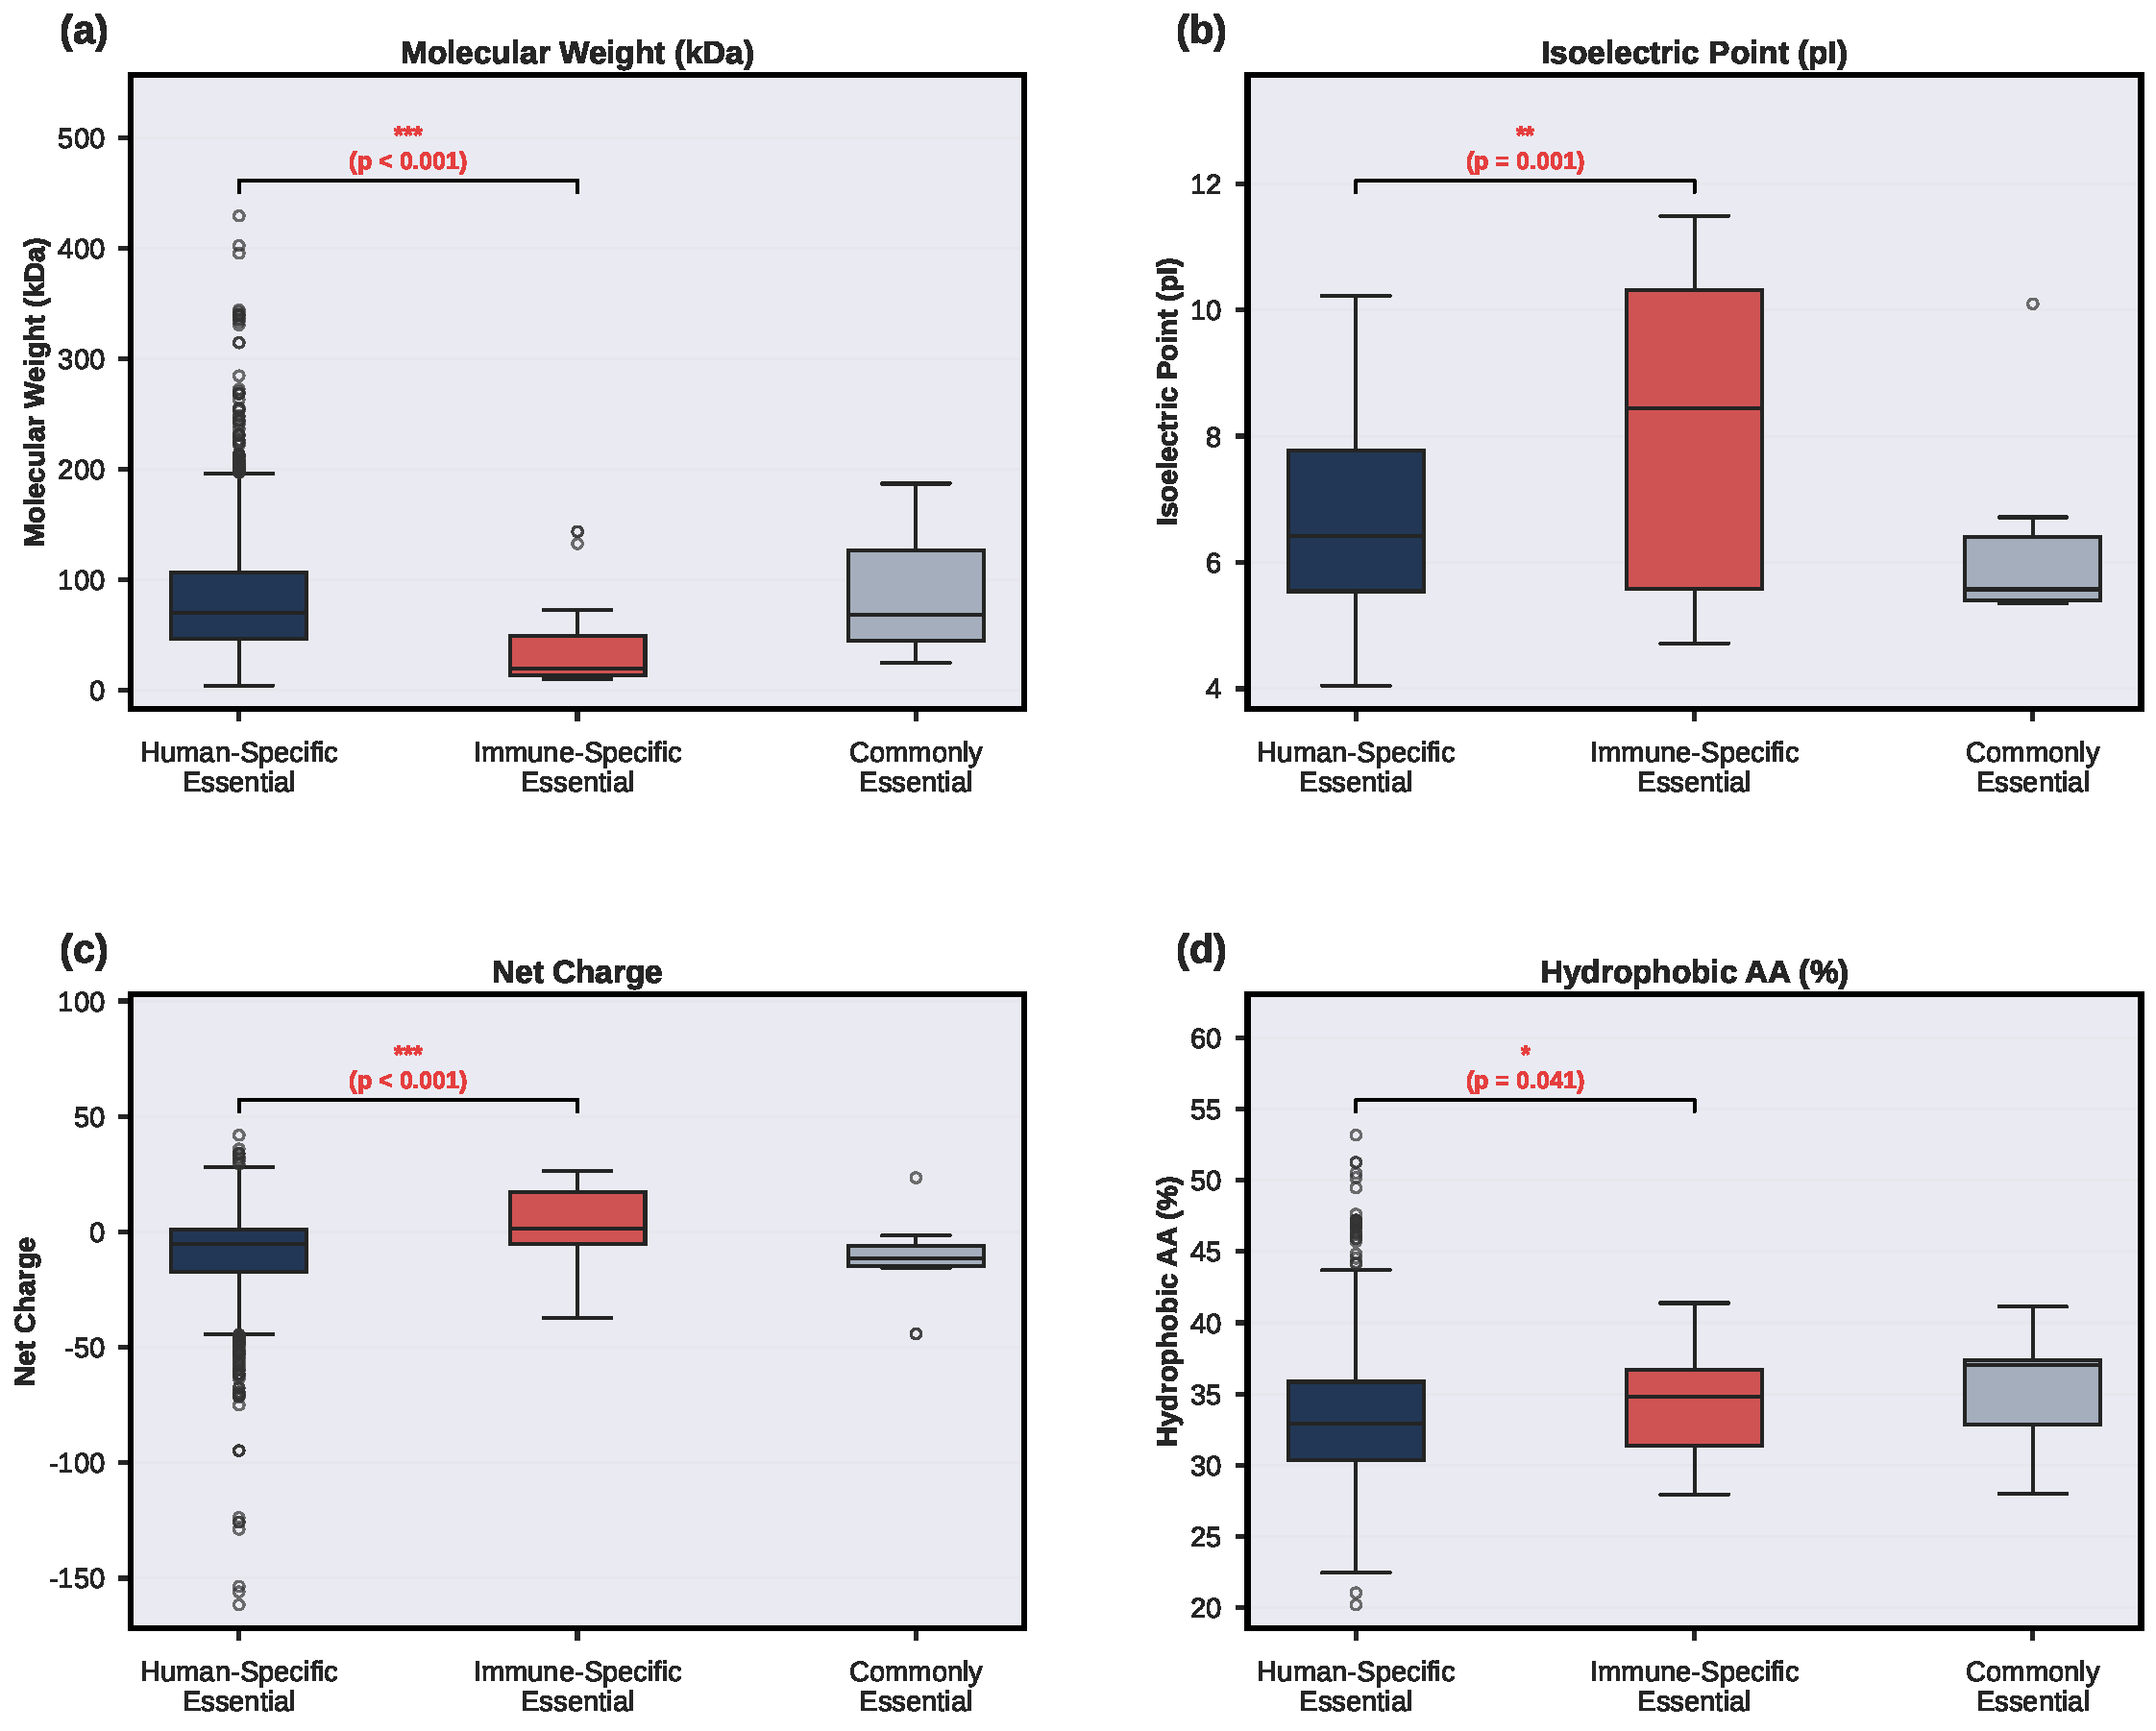
\includegraphics[width=0.98\linewidth]{figures/biophysical_features.pdf}
    \caption[不同蛋白分群的整体理化性质比较]{不同蛋白分群的整体理化性质比较，显示免疫情境候选必需蛋白整体呈现更轻量、更偏碱性且更具疏水性的理化特征。图中比较的三组分别为免疫情境候选必需蛋白、人类基础必需蛋白和共同必需蛋白。(a) 蛋白分子量分布；(b) 等电点分布；(c) 净电荷分布；(d) 疏水氨基酸比例分布。箱线图上方标示组间统计显著性。}
    \label{fig:biophysical_features}
\end{figure}

电荷属性的正向偏移是免疫情境候选必需蛋白最显著的统计特征之一。图~\ref{fig:biophysical_features}(b),(c) 显示，免疫情境候选必需蛋白 pI 明显升高（**$p=0.001$），同时净电荷（Net Charge）明显高于人类基础必需蛋白（***$p<0.001$）。具体而言，其 pI 的分布重心从中性区域向 pI 8.0--10.0 的碱性区间移动。该电荷重分布可能具有多层适应意义：在吞噬体酸化环境中，碱性蛋白更易维持功能所需的电荷状态与构象稳定性；正电表面可增强与带负电分子的静电相互作用，从而提高识别与结合效率；此外，在呼吸爆发过程中，多种蛋白复合体需进行快速、可逆组装，富含碱性残基的表面可能有助于增强瞬时电荷驱动的蛋白--蛋白相互作用。

最后，疏水氨基酸比例表现出统计学意义上的升高 (*$p=0.041$)。图~\ref{fig:biophysical_features}(d) 显示，免疫情境候选必需蛋白的疏水比例多集中在 45\% 至 55\% 之间。疏水残基比例的升高通常意味着蛋白内部折叠核心更加致密稳定。在高 ROS 环境中，强化的疏水核心可减少易氧化位点的暴露面积，提高整体热力学稳定性。同时，中性粒细胞功能涉及大量膜相关与脂质环境过程，适度增强的疏水区域亦可能有助于底物结合或膜界面相互作用。

综合氨基酸组成与整体理化参数的差异，可以观察到免疫情境候选必需蛋白在多个维度呈现协同偏移：结构轻量化、碱性增强、疏水核心强化以及极性残基减少。这些特征构成一种系统性的理化适应模式，显著契合中性粒细胞所处的酸化、氧化及高酶活性环境，提示免疫情境候选必需蛋白并非通用必需蛋白的随机子集，而是在特定免疫压力下形成的应激适应型蛋白集合。

\section{结构域富集与功能机制建模}

为系统解析不同必需蛋白亚群在分子层面的功能差异，本研究综合分析了结构域富集、功能关键词富集及亚细胞定位特征。整体趋势如图~\ref{fig:domain_enrichment}、图~\ref{fig:keyword_enrichment} 与图~\ref{fig:subcellular_localization} 所示，不同层级的必需蛋白在结构模块构成与功能指向上呈现出系统性分化，提示必需性并非简单来源于表达差异，而是对应于不同的分子功能架构与情境适配策略。

\begin{figure}[!htbp]
    \centering
    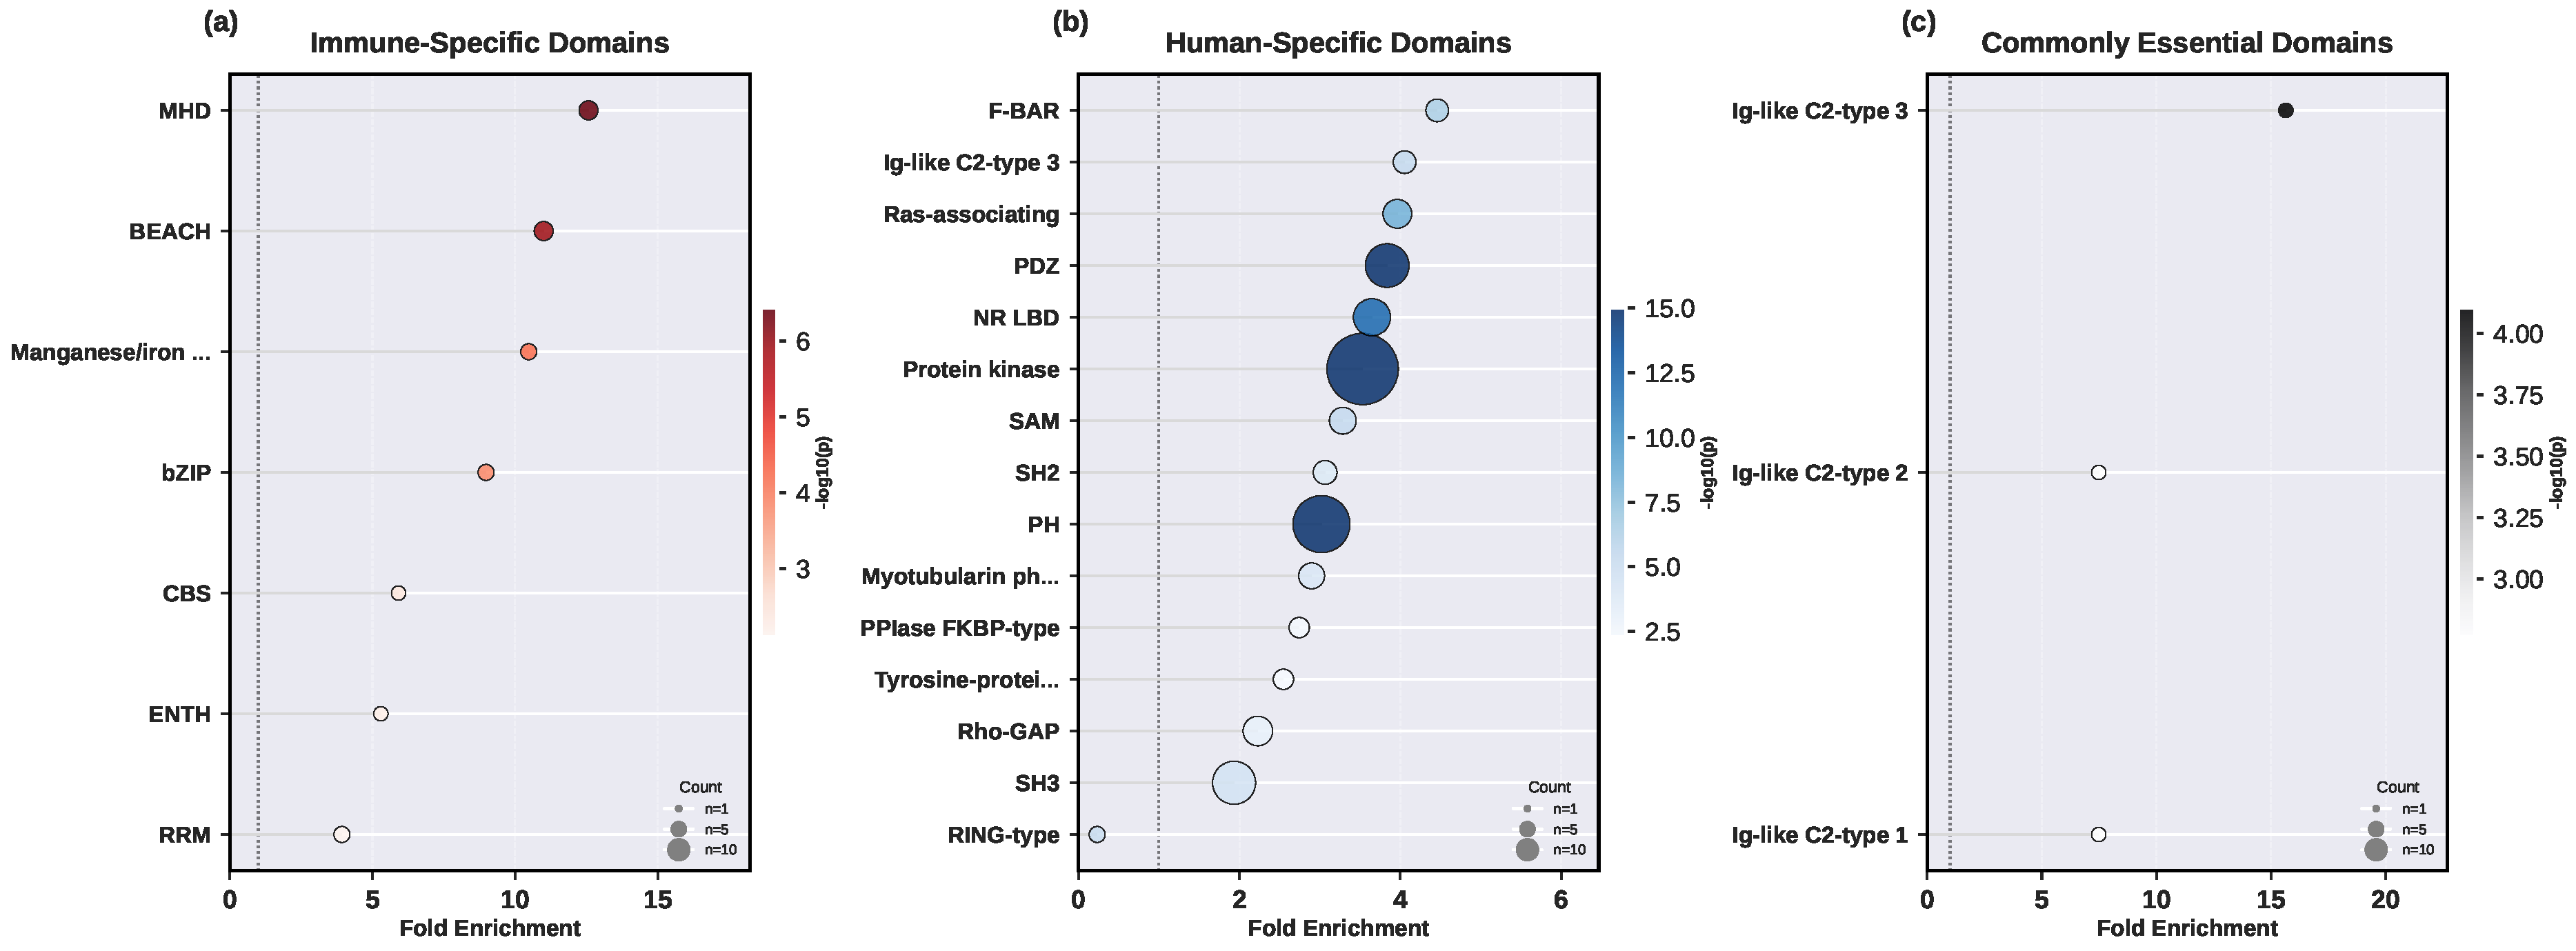
\includegraphics[width=0.98\linewidth]{figures/domain_enrichment.pdf}
    \caption[不同蛋白分群的结构域富集比较]{不同蛋白分群的结构域富集比较，揭示三类蛋白在功能模块组成上的系统性差异及潜在分工。(a) 免疫情境候选必需蛋白中显著富集的代表性结构域；(b) 人类基础必需蛋白中显著富集的代表性结构域；(c) 共同必需蛋白中显著富集的代表性结构域。}
    \label{fig:domain_enrichment}
\end{figure}
\begin{figure}[!htbp]
    \centering
    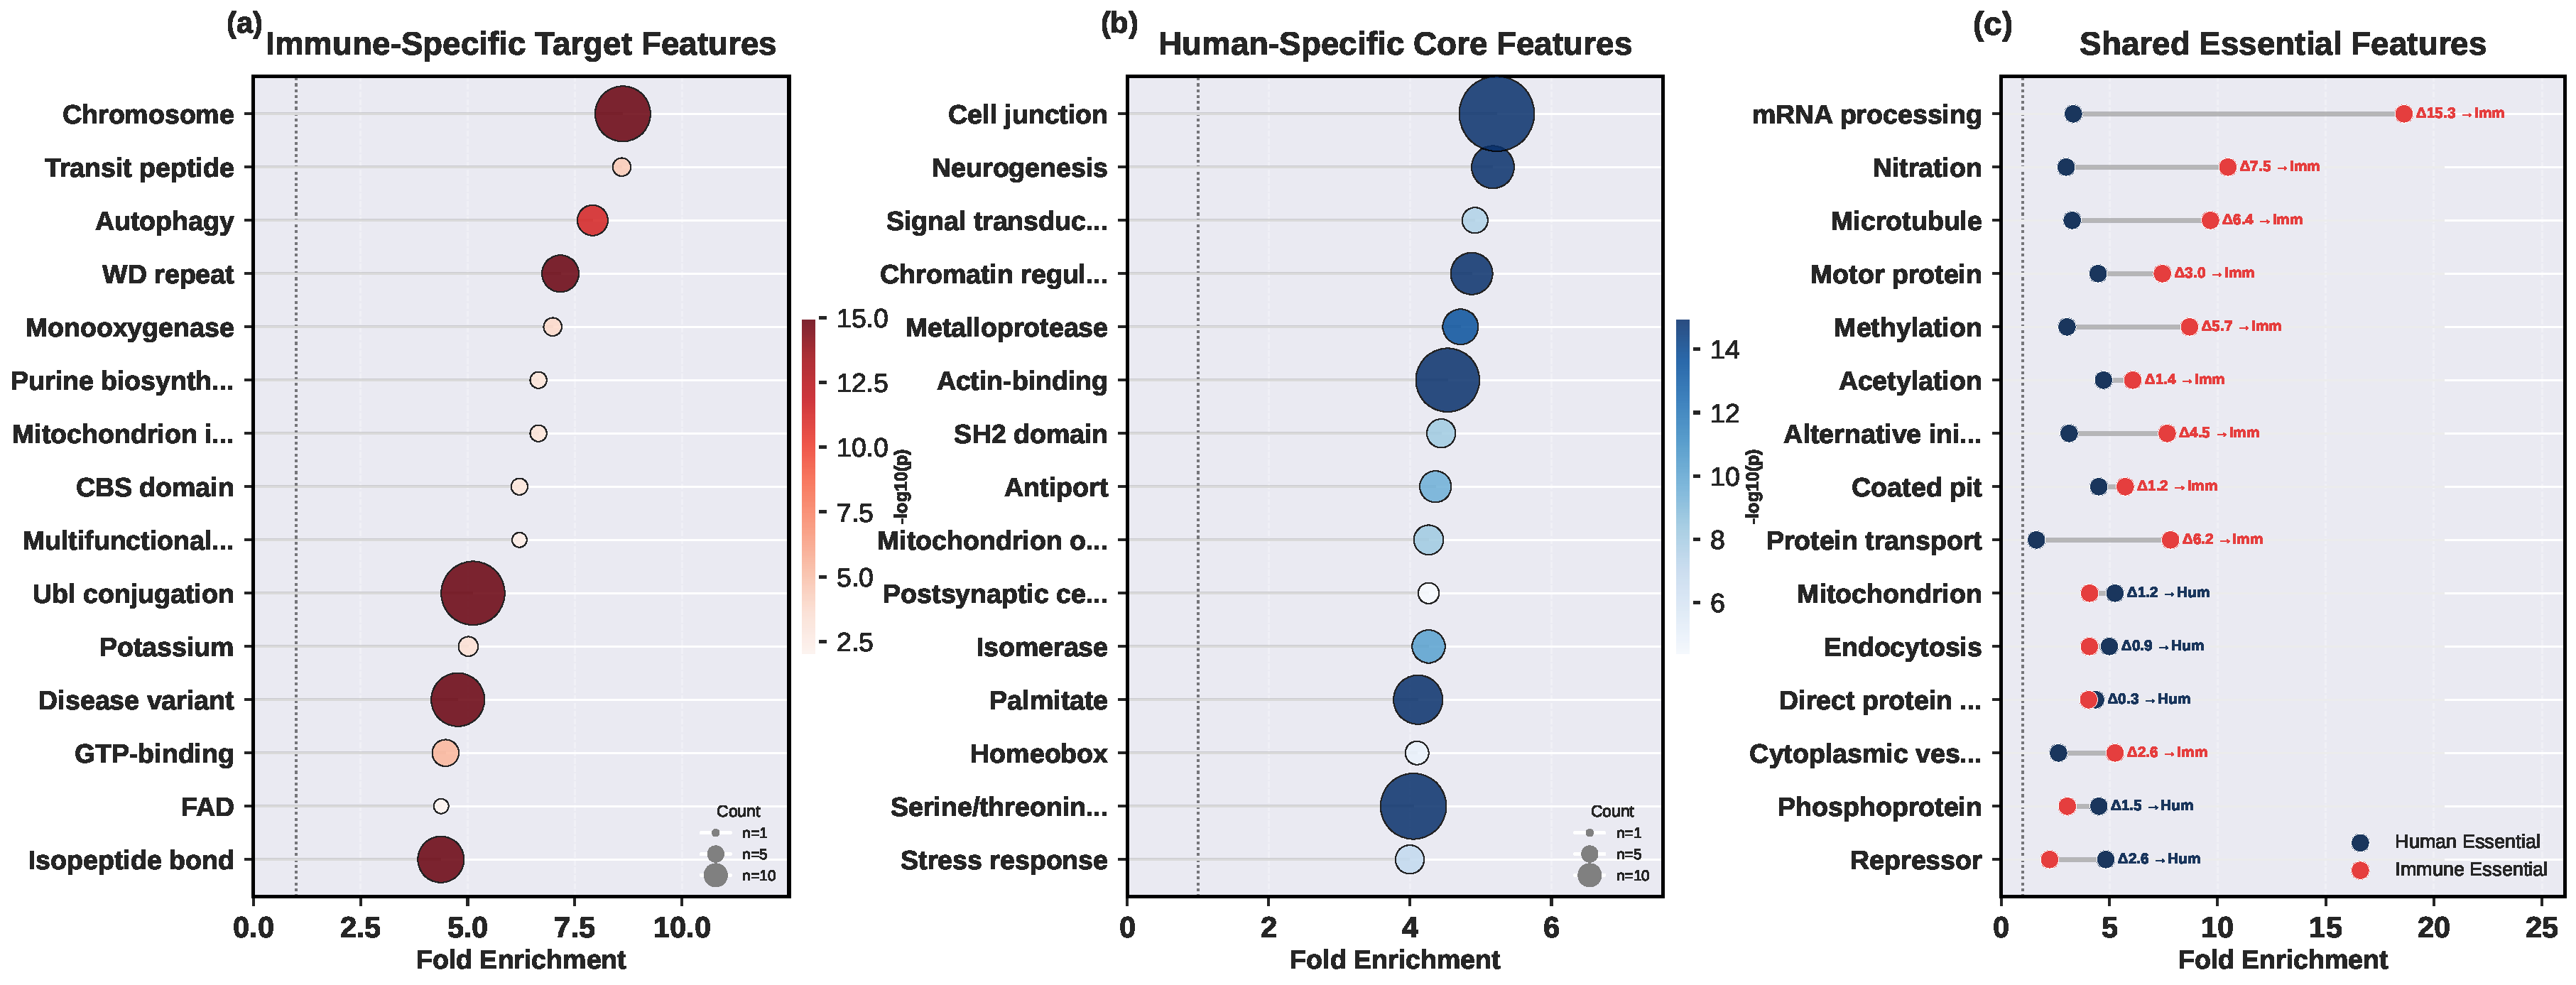
\includegraphics[width=0.98\linewidth]{figures/keyword_enrichment.pdf}
    \caption[不同情境下必需蛋白的功能关键词富集比较]{不同情境下必需蛋白的功能关键词富集比较，用于刻画不同情境下必需蛋白在应激响应、转录调控及细胞运输等功能上的依赖偏移。(a) 免疫情境中显著富集的功能关键词；(b) 人类整体背景中显著富集的功能关键词；(c) 两种情境均显著但富集方向或强度存在差异的共享关键词。}
    \label{fig:keyword_enrichment}
\end{figure}
\begin{figure}[!htbp]
    \centering
    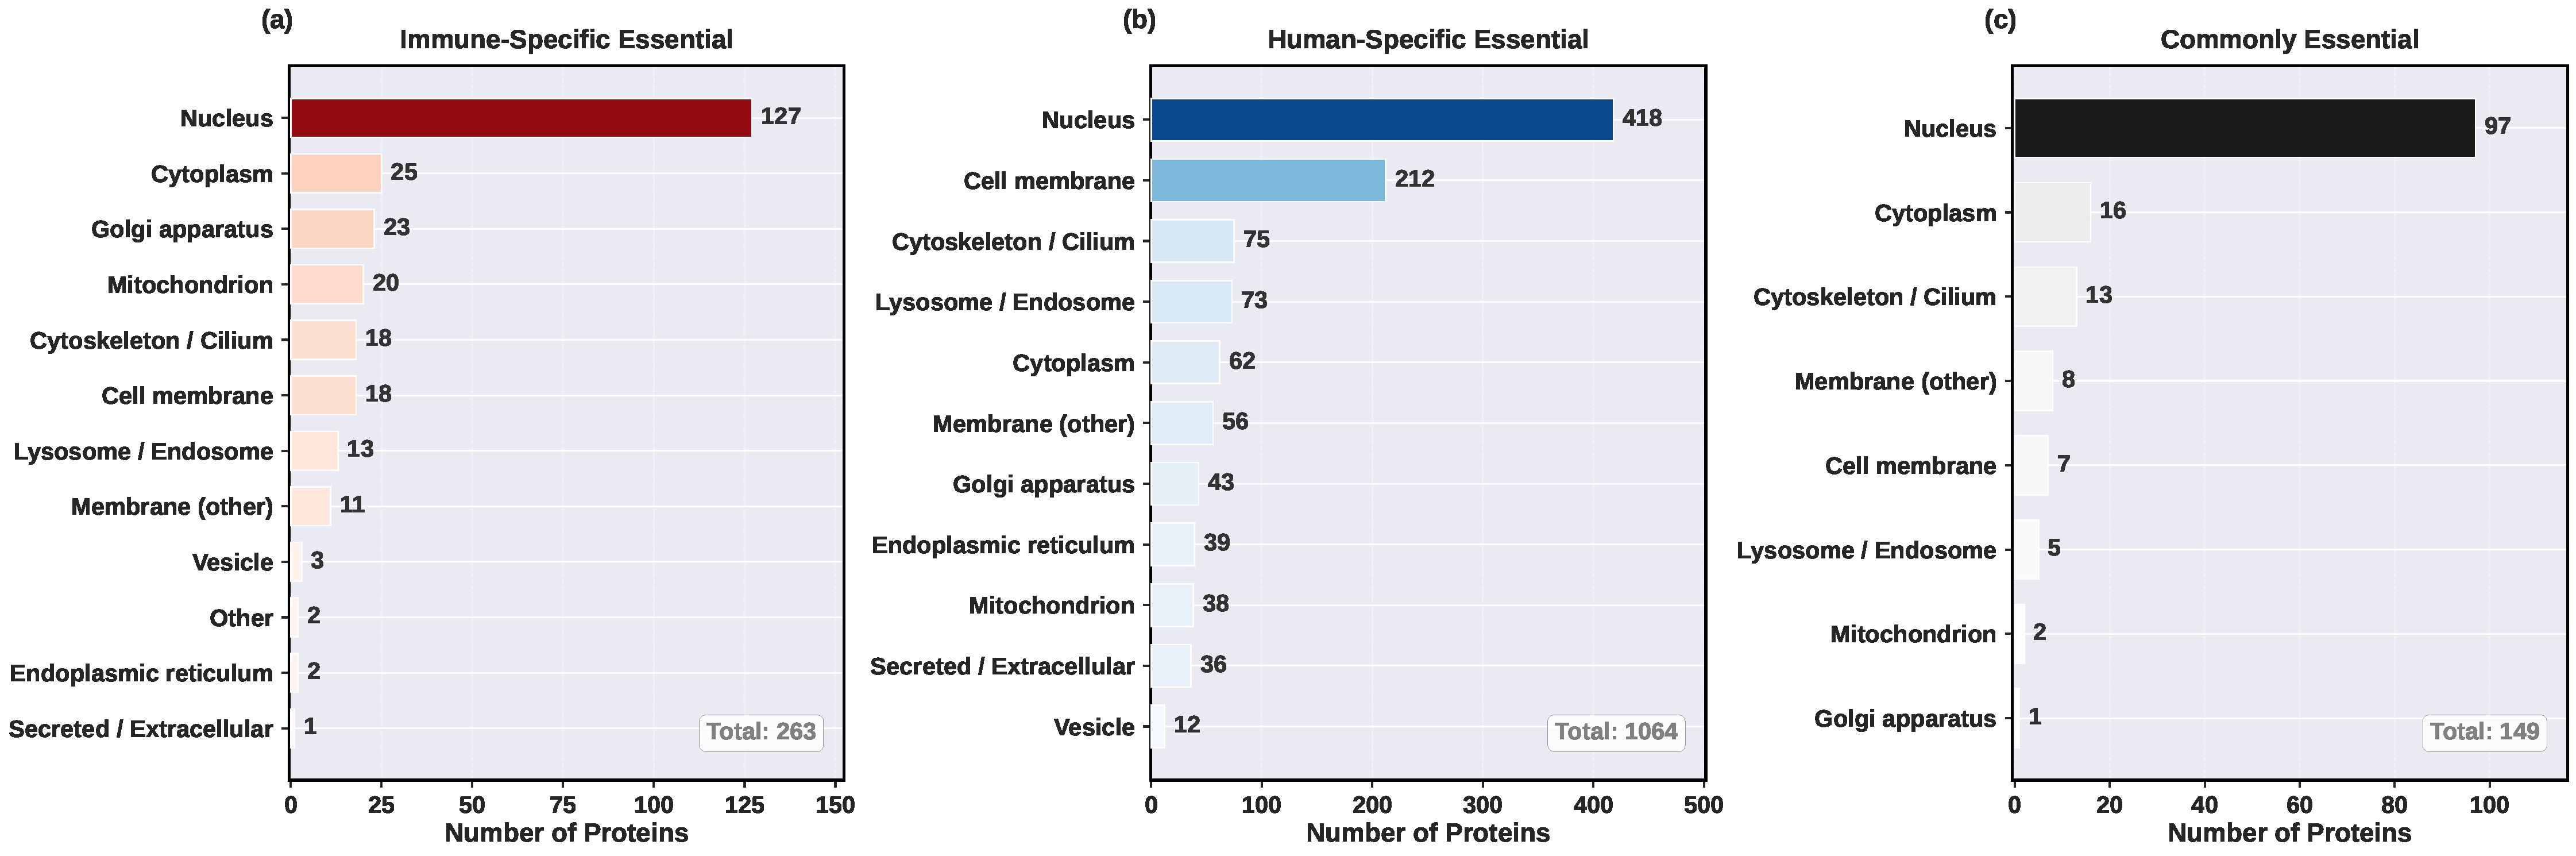
\includegraphics[width=0.98\linewidth]{figures/subcellular_localization.pdf}
    \caption[不同蛋白分群的亚细胞定位分布]{不同蛋白分群的亚细胞定位分布，显示免疫情境候选必需蛋白相较于人类基础必需蛋白更偏向线粒体与胞质相关区室，而人类基础必需蛋白则更集中于细胞核。(a) 免疫情境候选必需蛋白的亚细胞定位比例；(b) 人类基础必需蛋白的亚细胞定位比例；(c) 共同必需蛋白的亚细胞定位比例。}
    \label{fig:subcellular_localization}
\end{figure}

从结构域层面观察，如图~\ref{fig:domain_enrichment}(c) 所示，共同必需蛋白显著集中于 Ig-like C2-type 家族模块。该类结构域广泛参与细胞--细胞识别、膜受体相互作用及信号整合，在维持细胞结构稳定性与跨膜通讯中发挥基础性作用。结合图~\ref{fig:subcellular_localization}(c) 的定位分布可以看出，共同必需蛋白主要位于细胞核及胞质相关区域，提示其构成细胞结构与信号识别网络的基础骨架层。进一步对比图~\ref{fig:keyword_enrichment}(c) 可见，即便属于共享功能模块，其在不同情境下的富集强度仍存在方向性偏移，反映出共享通路内部的依赖权重重分配。

在人类基础必需组中，如图~\ref{fig:domain_enrichment}(b) 所示，Protein kinase、PH、SH2、PDZ 及 Ras-associating 等信号转导相关模块显著富集。相应地，图~\ref{fig:keyword_enrichment}(b) 显示其功能关键词主要集中于 chromatin regulator、transcription 与 signal transduction 等类别。从亚细胞定位来看，图~\ref{fig:subcellular_localization}(b) 清晰表明该组蛋白高度偏向细胞核区域。这些证据共同支持，人类基础必需蛋白构成维持个体发育与长期稳态的调控核心层，其必需性主要体现为对转录控制与信号级联节点的依赖。

相比之下，免疫情境候选必需蛋白呈现出更为显著的应激适配特征。如图~\ref{fig:domain_enrichment}(a) 所示，Mn/Fe SOD N-terminal、BEACH、MHD、bZIP、CBS 及 ENTH 等模块显著富集；图~\ref{fig:keyword_enrichment}(a) 进一步显示 autophagy、ubiquitin conjugation 与 mRNA processing 等功能在该组中更为突出。从亚细胞定位角度观察，图~\ref{fig:subcellular_localization}(a) 表明该组蛋白相较于人类基础必需组在核区域的比例相对降低，而在线粒体及胞质相关区室中的占比有所提高。Mn/Fe SOD N-terminal 结构域的富集提示其可能参与活性氧（ROS）清除与氧化还原稳态维持；结合自噬、膜重塑以及溶酶体相关模块的增强，可以推测该类蛋白更侧重于应激损伤缓冲与细胞器质量控制。基于上述富集趋势，可提出一个情境适配模型：ROS 生成增强 $\rightarrow$ 颗粒/溶酶体负荷升高 $\rightarrow$ 抗氧化与修复模块强化 $\rightarrow$ 自噬与膜运输系统维持损伤清除 $\rightarrow$ 细胞功能得以稳定。

尤为值得强调的是，共同功能模块在两种情境下呈现出方向性富集偏移。如图~\ref{fig:keyword_enrichment}(c) 所示，mRNA processing、microtubule 与 protein transport 在免疫情境下富集强度更高，而 repressor 等调控相关功能在人类整体层面偏好更强。这一现象揭示了“共同通路中的差异化依赖”，说明免疫适配并非通过引入全新通路实现，而是在既有基础通路内部重新分配关键步骤的依赖权重，从而实现情境特异的功能重构。

结构域、功能关键词与亚细胞定位的综合分析揭示了三类蛋白分群在功能层级上的系统分化：共同必需蛋白构成细胞结构与识别网络的基础骨架层；人类基础必需蛋白承担基因表达与信号放大的调控核心层；免疫情境候选必需蛋白则形成氧化还原稳态、自噬适配以及溶酶体负荷缓冲的应激保护层。该结构--功能分层模型为免疫情境相关依赖特征的分子基础提供了系统性解释，也为后续围绕氧化爆发-颗粒/溶酶体高负荷活化状态开展靶点筛选与机制验证奠定了理论框架。

通过对三类必需蛋白集合在分子量、电荷分布、结构域构成及亚细胞定位等多维度特征的系统比较，本章识别出一组在种群层面相对耐受、但在免疫细胞应激执行过程中表现出高度依赖性的候选蛋白。这些蛋白所呈现的理化适应模式与中性粒细胞特有的酸化环境及氧化应激状态高度契合，为其潜在功能重要性提供了结构层面的解释。

基于上述筛选结果，下一章将选取其中具有代表性的候选蛋白，开展结构解析与功能验证，以构建从计算预测到实验验证的完整研究闭环。

\section{核心候选蛋白的注意力图谱解析与结构域功能验证}

在完成对免疫情境候选必需蛋白的群体理化特征分析后，本小节旨在通过深度学习模型的注意力机制，对最终筛选出的核心候选蛋白进行位点层面的深度解析。通过提取模型在预测 $\text{PES}_{\text{immune}}$ 评分时的注意力权重分配，可以精确识别出序列中对 Immune-level 依赖判定贡献最大的关键残基。这种从“整体统计”向“单分子位点”的解析过渡，不仅能够验证模型预测的生物学合理性，更能揭示这些蛋白在中性粒细胞应激环境下的功能执行基础。

本研究选取了筛选结果中具有代表性的核心候选蛋白（如 $\text{ATP6V1A}$、$\text{ATP6V1B2}$、$\text{H2BC11}$ 及 $\text{PLBD1}$），通过自注意力热图、归一化重要性曲线、氨基酸理化特征轨以及已知功能结构域四个维度的信息分析这些特征在序列空间上的协同分布，探讨模型判定其为免疫情境候选必需靶点的数理与生物学依据。注意力热图是揭示蛋白内部空间相互作用逻辑与全局关联特征的核心特征，通过热力图的形式展示了序列中任意两个残基之间的关联程度，反映了模型对蛋白质空间折叠与功能协同的表征能力。归一化重要性曲线通过量化表征序列中每一个氨基酸残基对 $\text{PES}_{\text{immune}}$ 的边际贡献权重，揭示了蛋白质执行特定免疫功能时的关键位点分布特征，深色覆盖区域代表了该蛋白质中已被科学界确认存在的已知功能域。疏水序列轨定量化地展示蛋白质序列随氨基酸位置变化而产生的“疏水性/亲水性”交替分布特征，反映了模型对蛋白质空间拓扑结构（如内部核心或膜界面）的学习能力。底端的电荷序列轨是揭示蛋白功能微环境的关键维度，通过颜色梯度展示氨基酸残基在生理 pH（pH 7.0）下的带电状态，绿色代表正电荷，紫色代表负电荷，而白色则代表中性或非极性区域。

\paragraph{1. 吞噬体酸化相关的 V-ATPase 复合体亚基解析}
V-ATPase 是维持中性粒细胞吞噬体酸化的重要蛋白复合体，其功能状态直接决定了杀菌微环境的 pH 值稳态。如图 \ref{fig:atp6v1a} 所示，$\text{ATP6V1A}$（A 亚基）的归一化重要性峰值主要分布于其 $\text{V-ATPase A consensus}$ 已知功能域内。模型识别出的关键特征位点包括 $\text{W354}$、$\text{M368}$、$\text{F417}$、$\text{Q430}$ 及 $\text{W450}$。

注意力热图（Attention Map）进一步揭示了复杂的残基交互逻辑：核心节点 $\text{W354}$ 表现出显著的长程关联性，与序列前端的 $\text{K8}$、$\text{S111}$ 以及末端的 $\text{S500}$ 存在强注意力交互。结合底端的理化分布轨可以发现，这些高权重位点在序列空间上展现出显著的理化特征耦合，即重要性峰值多定位于电荷富集区，并与疏水性的局部分布模式高度吻合。

\begin{figure}[!htbp]
    \centering
    \makebox[\linewidth][c]{\rotatebox{90}{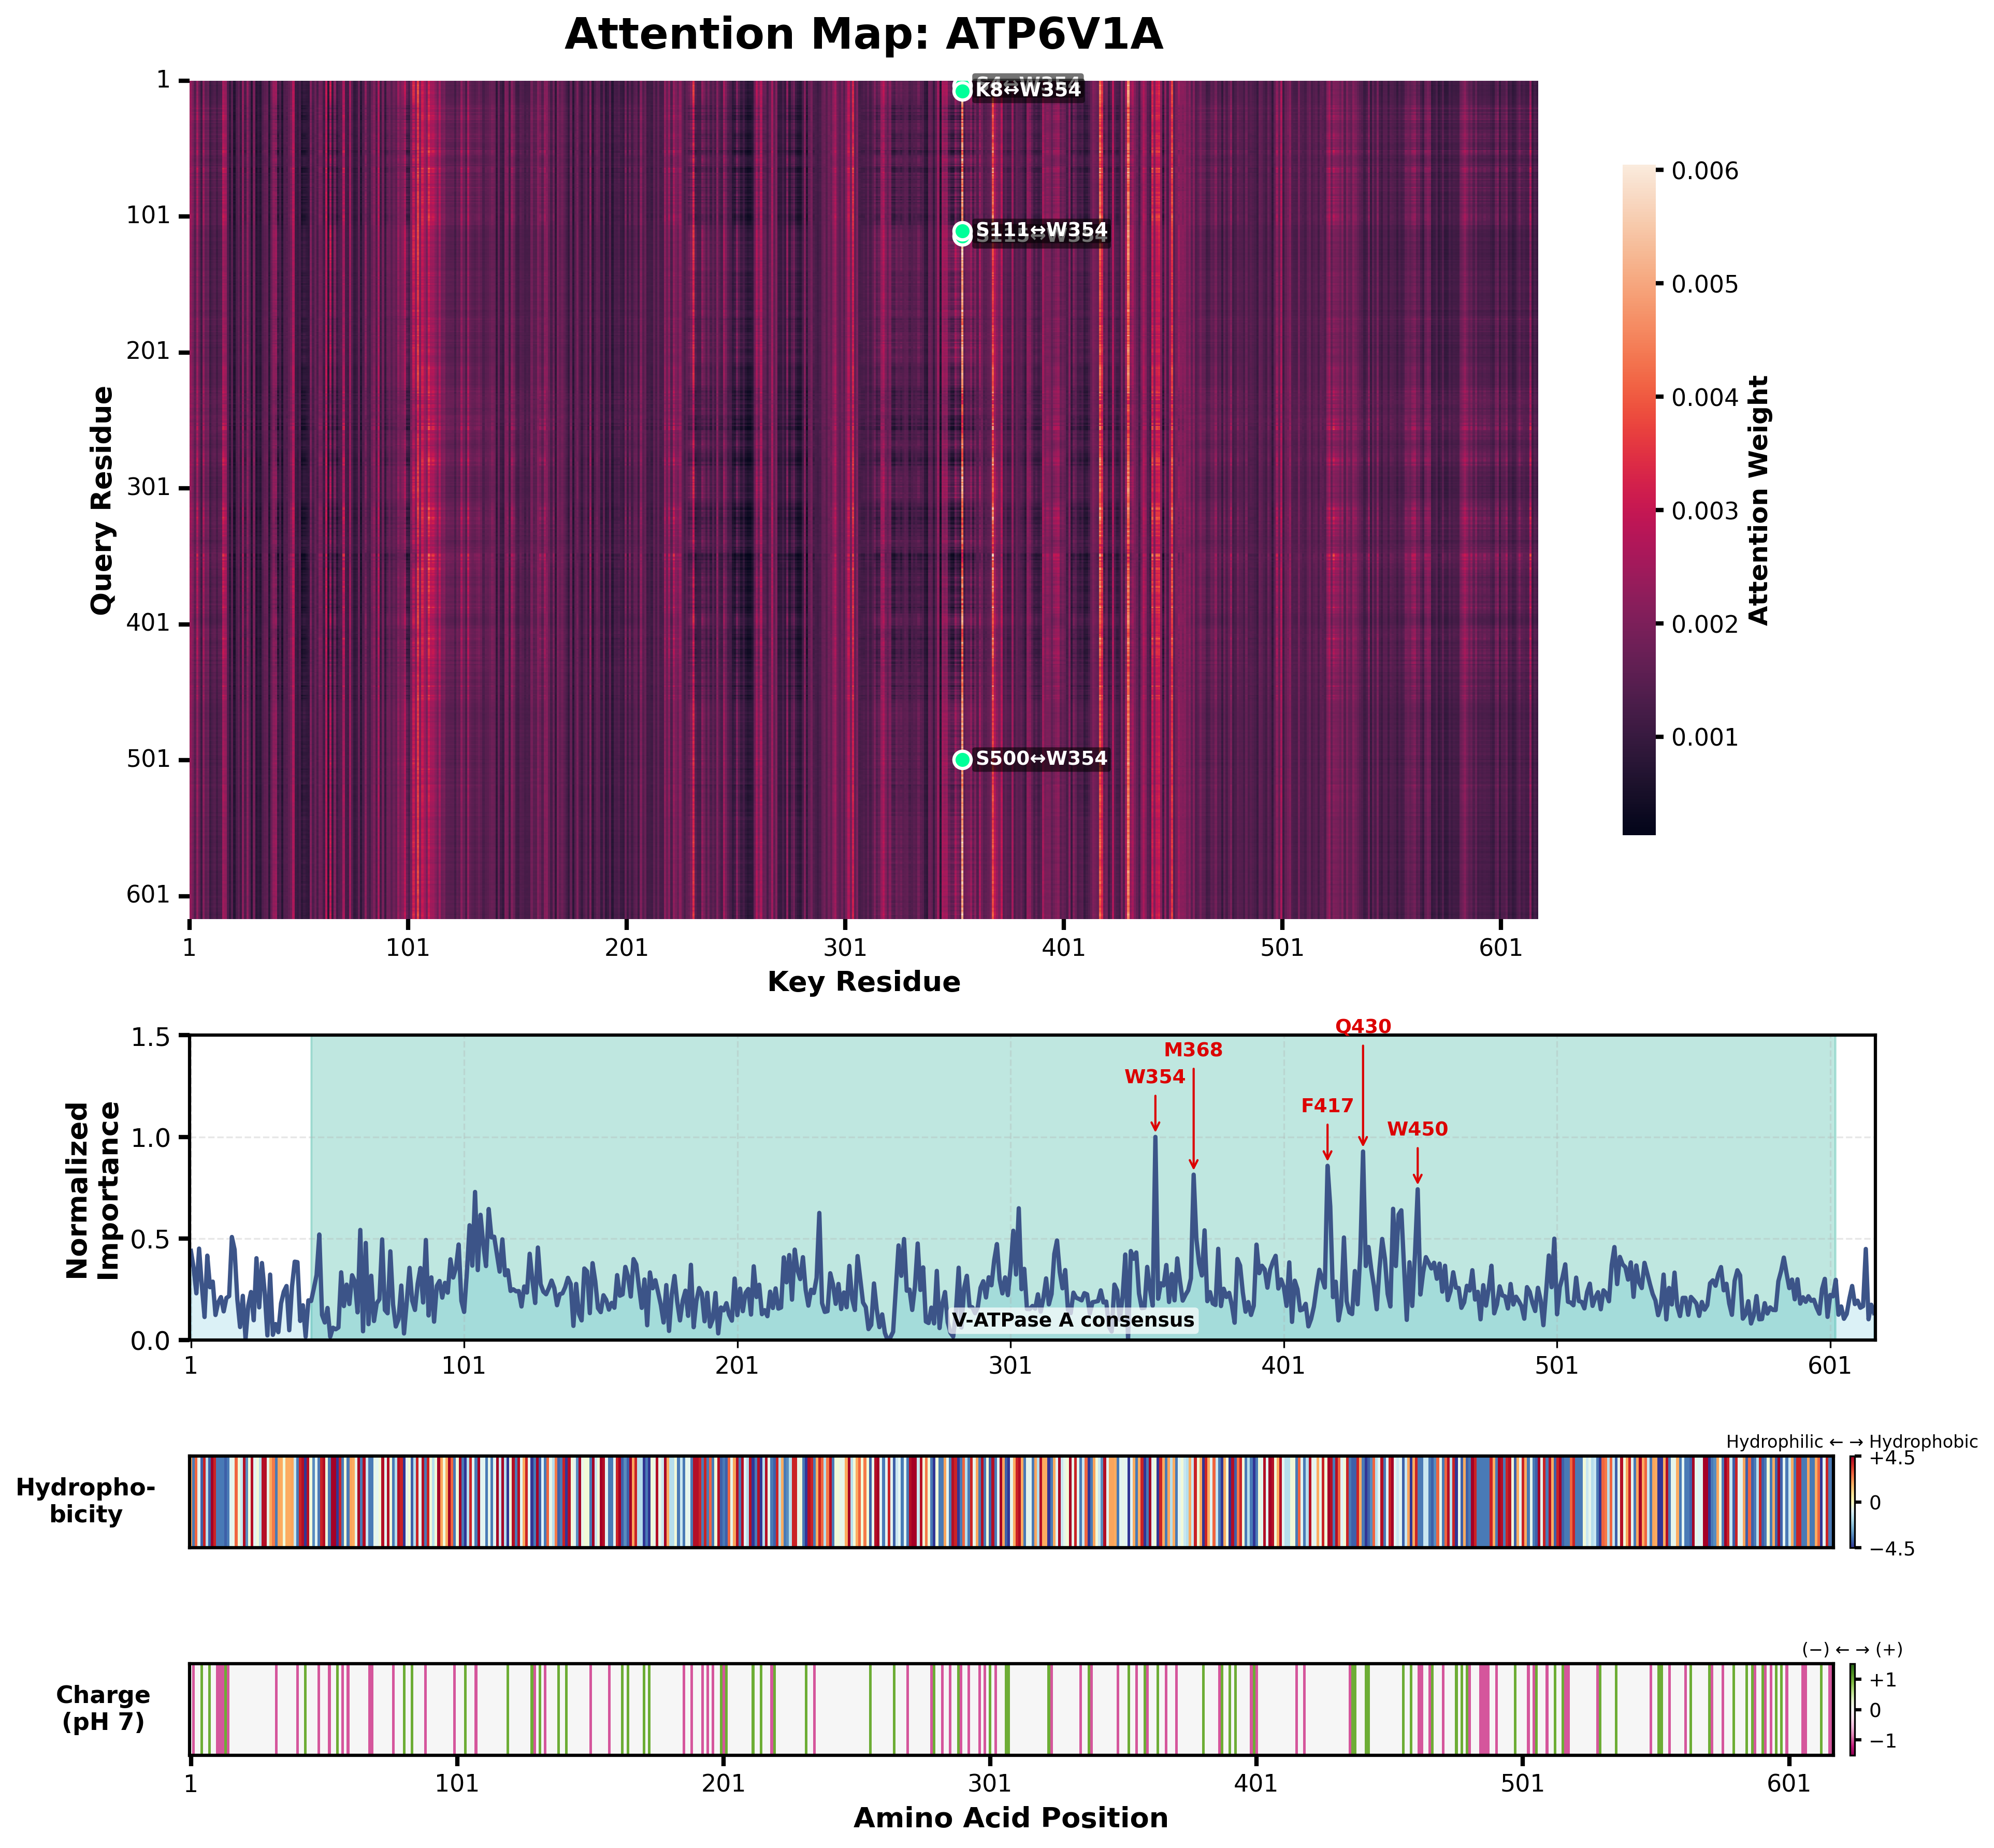
\includegraphics[width=0.72\textheight]{figures/ATP6V1A_dense.png}}}
    \caption[$\text{ATP6V1A}$ 的深度注意力机制可视化]{$\text{ATP6V1A}$ 的深度注意力机制可视化。图中整合了残基间自注意力热图、归一化重要性曲线及序列理化轨迹，显示模型高权重位点与已知功能域及局部电荷环境具有良好对应关系。}
    \label{fig:atp6v1a}
\end{figure}

与之对应的 $\text{ATP6V1B2}$ 亚基展现了类似的“结构域导向”特征（图 \ref{fig:atp6v1b2}）。其重要性权重高度富集于 $\text{V-ATPase B consensus}$ 已知功能域区域。其中 $\text{S92}$ 被识别为贡献度最高的特征残基，并与 $\text{E70}$、$\text{Q97}$ 及 $\text{G173}$ 等位点形成了紧密的自注意力交互网络。其他显著峰值如 $\text{T46}$、$\text{F150}$、$\text{S216}$ 和 $\text{V317}$ 进一步完善了模型对该亚基必需性的判定依据。这种对 V-ATPase 关键催化亚基的高权重分配，表明模型能够在复杂序列背景下识别与中性粒细胞酸化功能相关的关键区域。

\begin{figure}[!htbp]
    \centering
    \makebox[\linewidth][c]{\rotatebox{90}{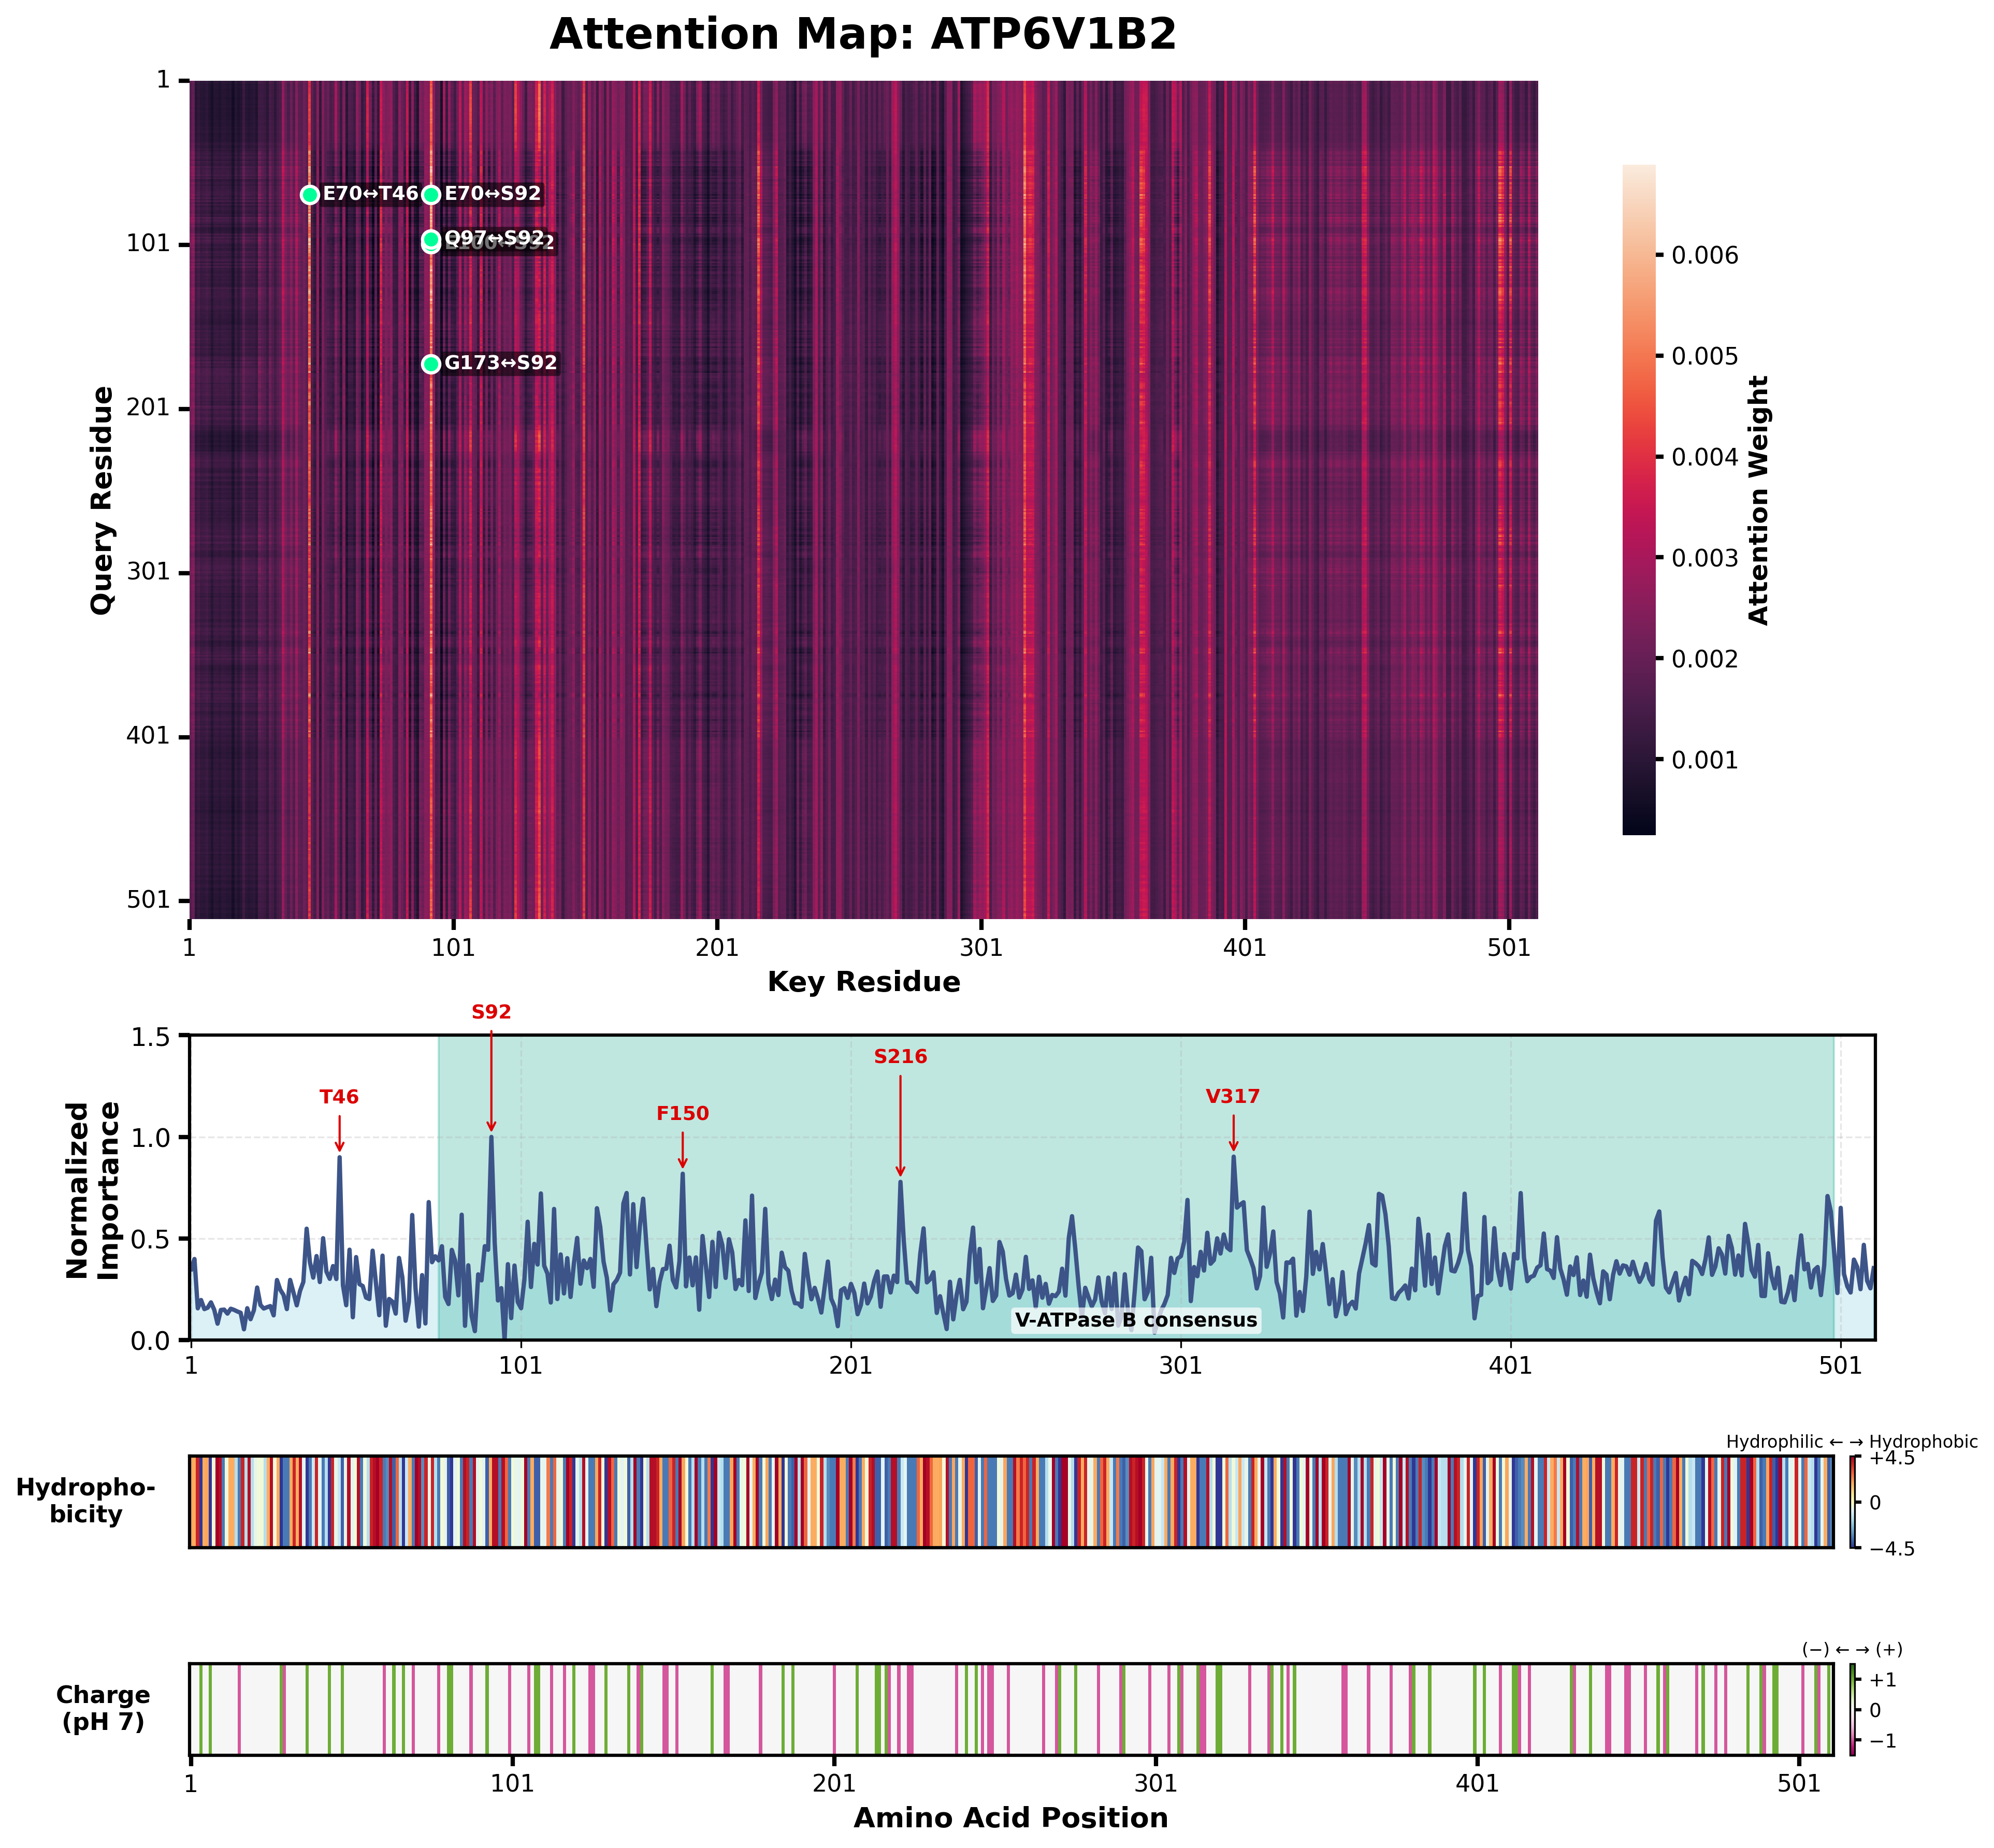
\includegraphics[width=0.67\textheight]{figures/ATP6V1B2_dense.png}}}
    \caption[$\text{ATP6V1B2}$ 的深度注意力机制可视化]{$\text{ATP6V1B2}$ 的深度注意力机制可视化。图中展示了关键残基的注意力关联模式、重要性峰值及其对应的疏水性与电荷分布，说明模型对 V-ATPase 功能核心区域具有显著聚焦。}
    \label{fig:atp6v1b2}
\end{figure}

\FloatBarrier
\paragraph{2. 染色质重塑与代谢功能蛋白：H2BC11 与 PLBD1}
组蛋白 $\text{H2BC11}$ 是中性粒细胞形成 NETs 的关键组分。其注意力图谱（图 \ref{fig:h2bc11}）显示，高权重位点高度富集于 $\text{Histone H2B}$ 已知核心功能域内。归一化曲线标定了 $\text{Y84}$、$\text{S88}$、$\text{H110}$、$\text{S113}$ 及 $\text{T120}$ 等关键突刺。

值得注意的是，$\text{S113}$ 位点作为关键节点，与 $\text{Q96}$、$\text{R100}$、$\text{L107}$ 以及序列末端的 $\text{K121}$、$\text{K126}$ 产生了显著的协同贡献（Query-Key 交互点）。理化分布轨显示，这些位点多位于强正电荷区间，这与其在 NETs 形成过程中需要适应中性粒细胞脱颗粒所伴随的离子强度变化、并维持染色质解聚与结构稳态的功能需求相一致。

\begin{figure}[!htbp]
    \centering
    \makebox[\linewidth][c]{\rotatebox{90}{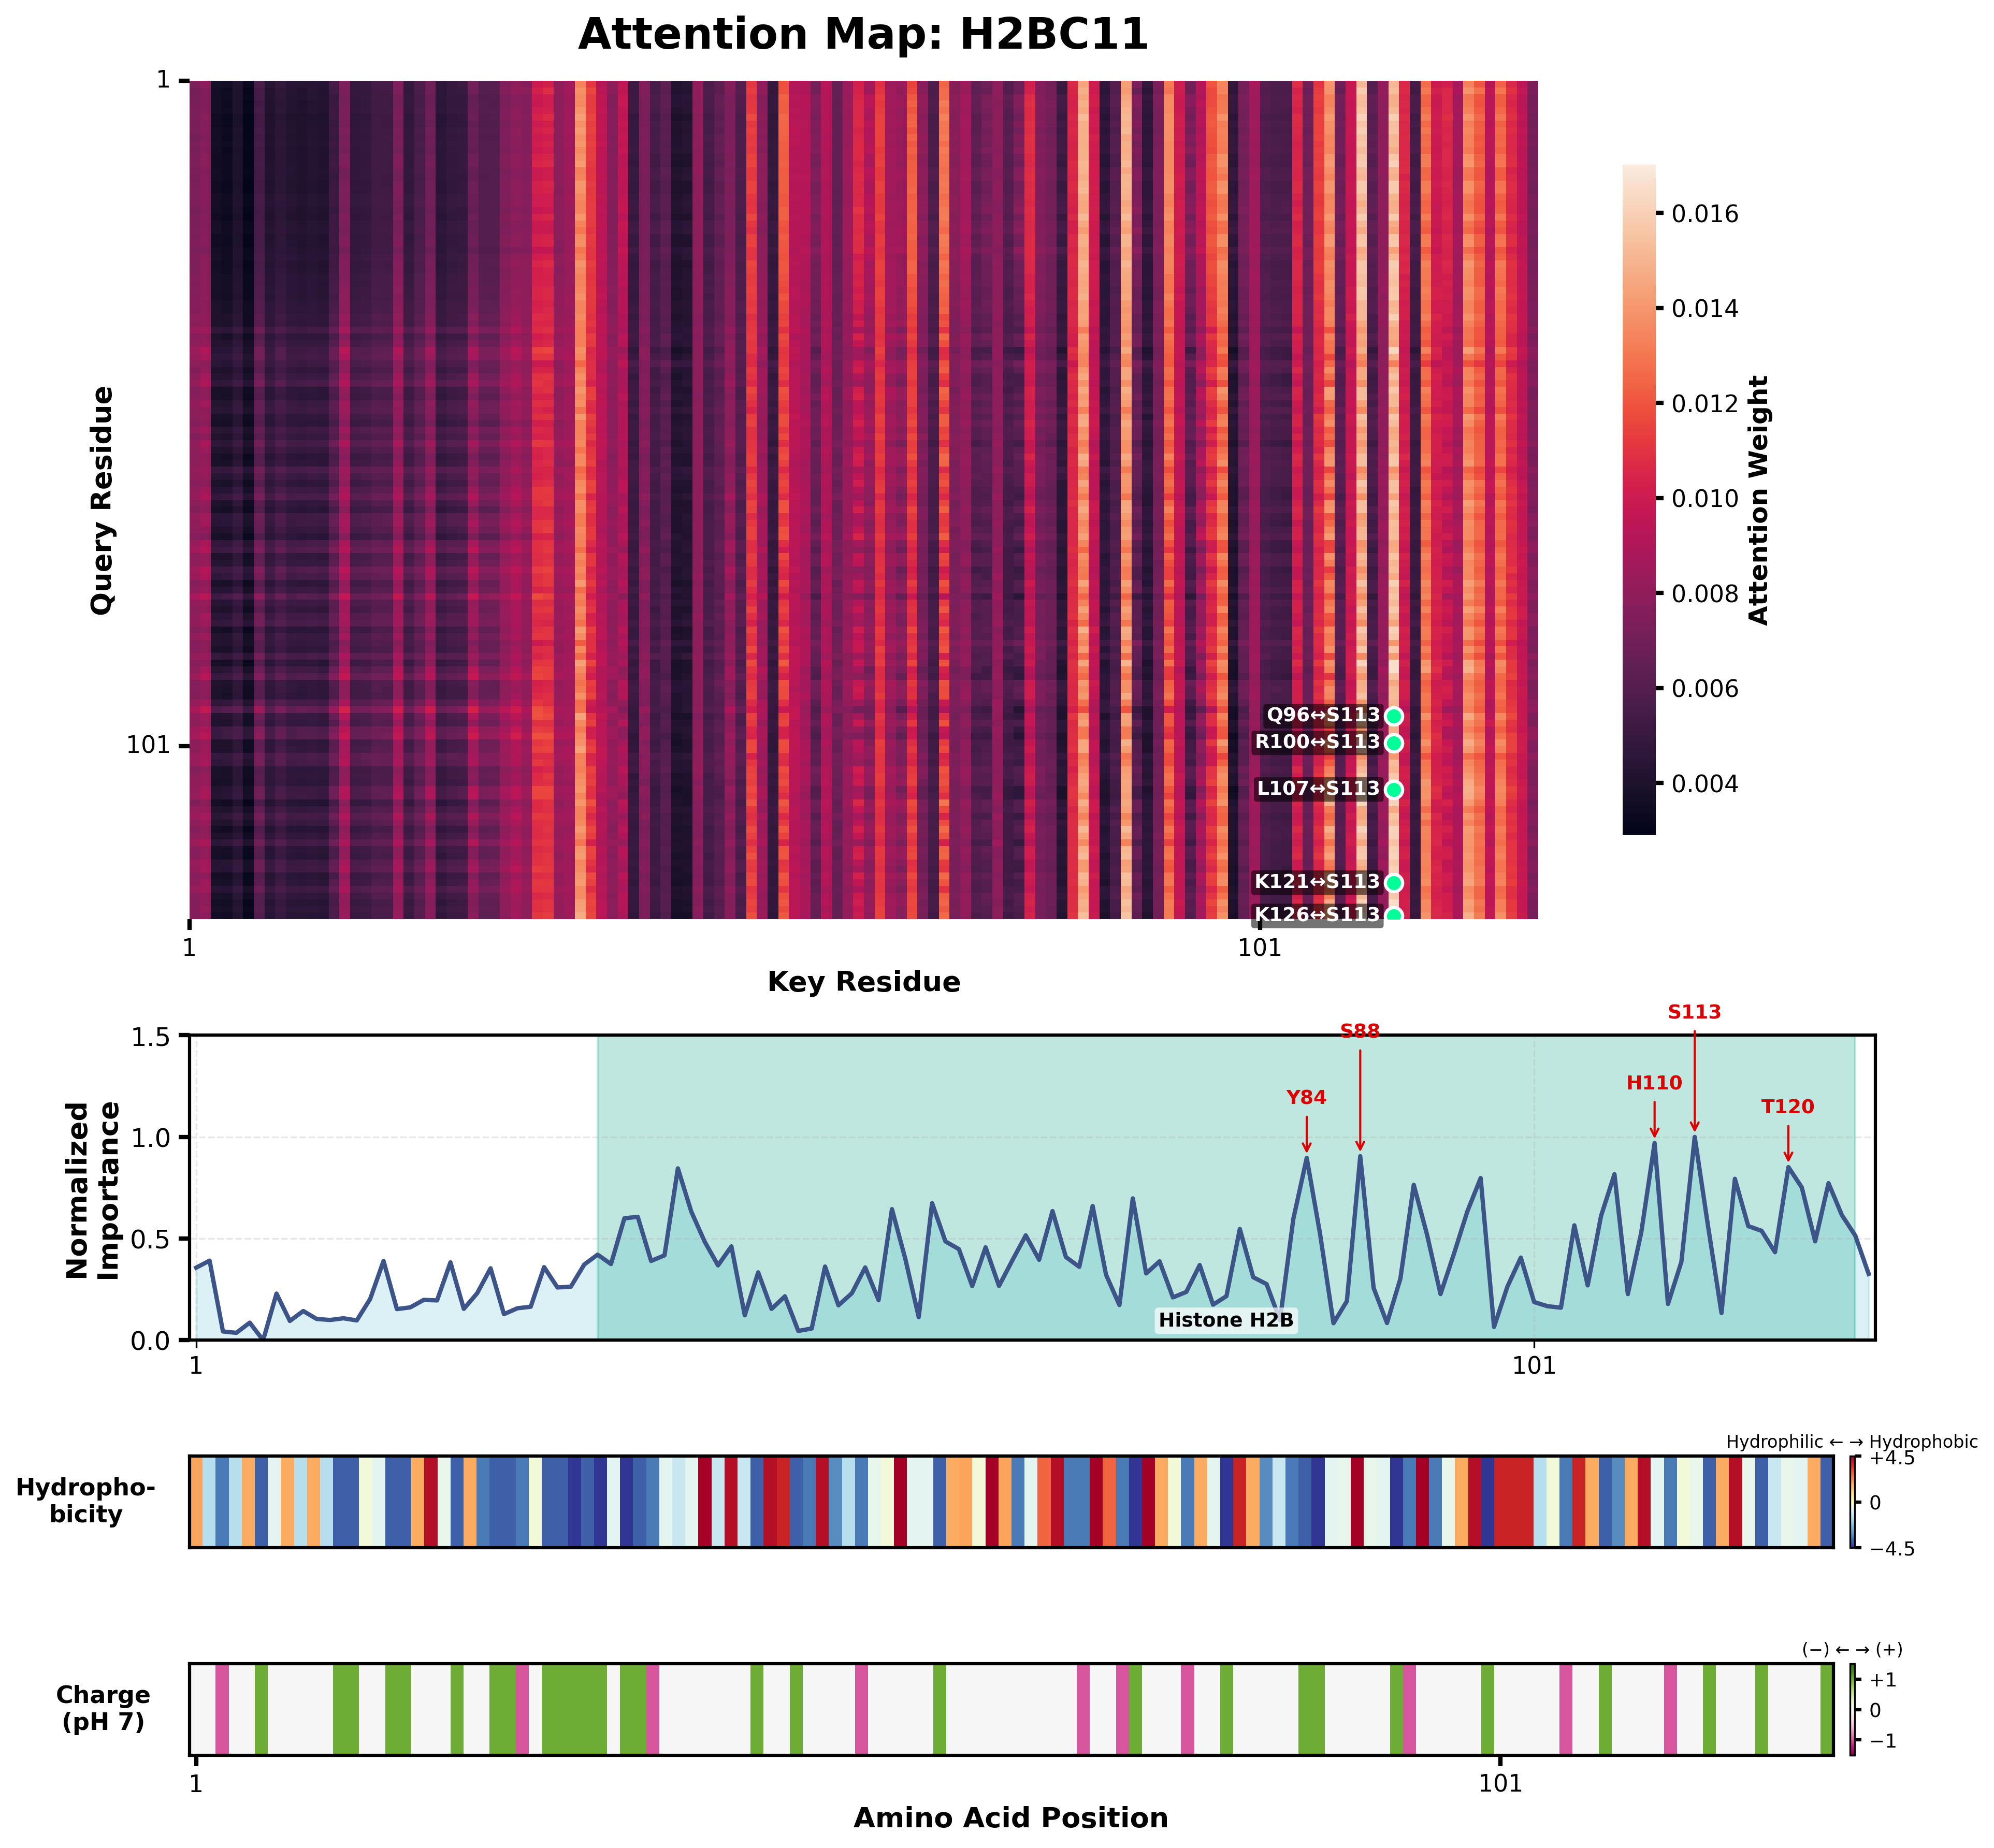
\includegraphics[width=0.67\textheight]{figures/H2BC11_dense.png}}}
    \caption[$\text{H2BC11}$ 的深度注意力机制可视化]{$\text{H2BC11}$ 的深度注意力机制可视化。图中综合展示组蛋白序列内部的注意力热点、残基重要性变化及理化性质分布，突出模型识别出的高权重点与功能域及强带电区段之间的对应关系。}
    \label{fig:h2bc11}
\end{figure}

磷脂酶 $\text{PLBD1}$ 的分析则揭示了模型对膜相关代谢蛋白的解析逻辑。如图 \ref{fig:plbd1} 所示，其重要性位点分布涵盖了 $\text{Phospholipase B-like}$ 已知功能域的多个基序，如 $\text{M60}$、$\text{S157}$、$\text{Q314}$、$\text{S368}$ 及 $\text{T445}$。与前述蛋白不同，$\text{PLBD1}$ 的注意力权重主要映射在疏水性较强的结构域区间，反映了模型对该蛋白在中性粒细胞溶酶体及膜脂代谢中功能定位的有效识别。关于 $\text{PLBD1}$ 在中性粒细胞生理病理过程中的具体作用机制，将在第四章展开详细论述。

\begin{figure}[!htbp]
    \centering
    \makebox[\linewidth][c]{\rotatebox{90}{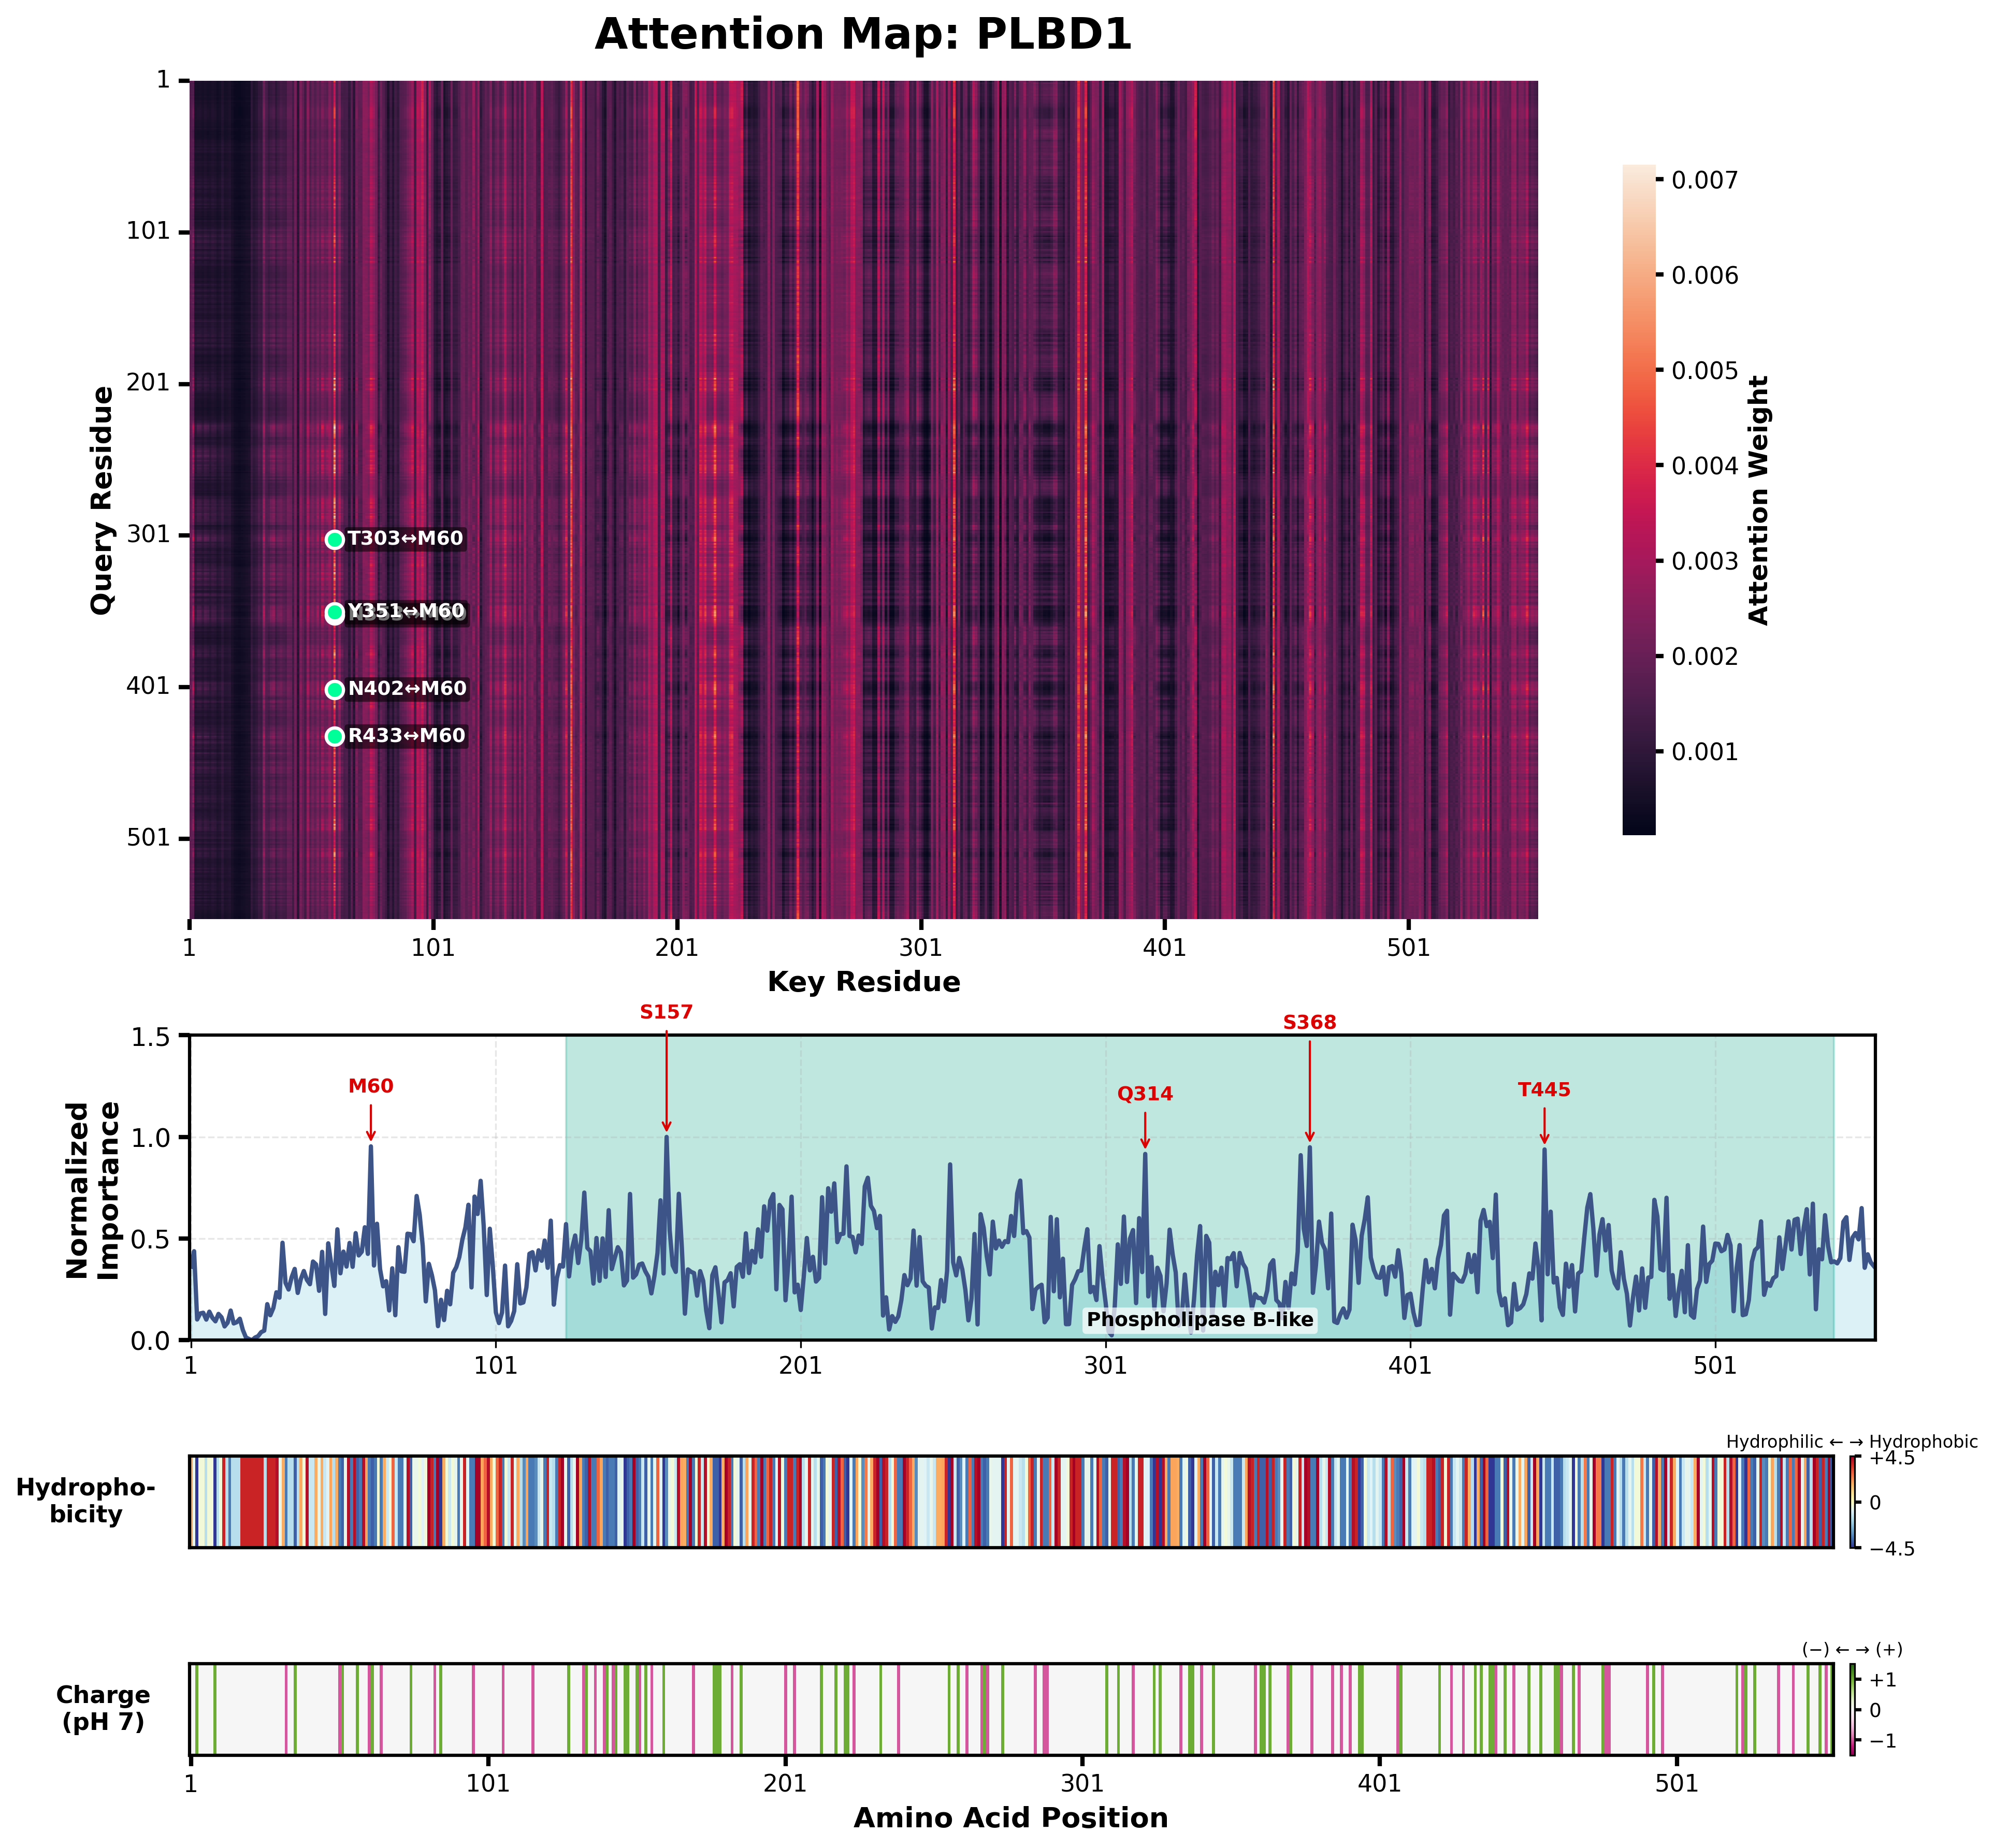
\includegraphics[width=0.67\textheight]{figures/PLBD1_dense.png}}}
    \caption[$\text{PLBD1}$ 的深度注意力机制可视化]{$\text{PLBD1}$ 的深度注意力机制可视化。图中同时呈现注意力热图、重要性曲线及序列理化轨迹，显示模型关注位点与疏水结构域及潜在功能区域之间具有明确的空间对应。}
    \label{fig:plbd1}
\end{figure}

综合上述典型蛋白的解析结果，可以发现模型提取的重要性位点与本章第二节中统计得出的系统性理化偏移之间逻辑统一：
\begin{itemize}
    \item \textbf{功能域映射的一致性}：归一化重要性峰值与已知功能域的高度重合，证明了模型判定依据的生物学严谨性，即必需性评分源于对核心功能结构域的识别。
    \item \textbf{理化特征的微观验证}：模型在 $\text{ATP6V1A}$ 等蛋白中捕捉到的高电荷位点，以及在 $\text{PLBD1}$ 中捕捉到的强疏位点，分别在单分子位点层面验证了前文所述的“碱性增强”与“疏水核心强化”等进化适应特征。
\end{itemize}

综上所述，通过注意力机制解析，本研究不仅从数理层面证实了筛选出的核心候选蛋白在已知功能结构域上的重要性，更明确了一系列关键的功能贡献残基。这些位点不仅是模型判定的数理支撑，也为后续第四章中针对 $\text{ATP6V1B2}$ 与 $\text{PLBD1}$ 等蛋白开展详细的功能机制探讨奠定了位点层面的研究基础。进一步看，从群体层面的理化统计偏移到单蛋白层面的关键位点聚焦，模型所给出的证据链条具有较好的层次一致性，说明其判别结果并非来源于孤立的表面模式，而是建立在多尺度结构与功能线索的综合整合之上。由此，注意力图谱不仅提升了预测结果的可解释性，也为后续实验中候选位点的优先级排序、突变设计以及机制假设的提出提供了直接依据。
